		%%%%%%%%%%%%%%ATTENTION%%%%%%%%%%%%%%%
		%%%%%!!!Use Biber and pdflatex!!!%%%%%
		%%%%%%%%%%%%%%ATTENTION%%%%%%%%%%%%%%%
% This Template was designed using MikTeX and TeXstudio.

		%%%%%%%%%%%%%%%ACHTUNG%%%%%%%%%%%%%%%%
		%%!!!Biber und pdflatex verwenden!!!%%
		%%%%%%%%%%%%%%%ACHTUNG%%%%%%%%%%%%%%%%
% Diese Vorlage wurde mit MikTeX und TeXstudio erstellt.


%%%%%%%%%%%%%%%%%%%%%%%%%%%%%%%%%%%%%%
%%%%%%%%%%%%%% Präambel %%%%%%%%%%%%%%
%%%%%%%%%%%%%%%%%%%%%%%%%%%%%%%%%%%%%%
%The preamble is the part of your document where all required packages and macros can be defined. This needs to be done before the \begin{document} command.
%MAKE YOURSELF FAMILIAR WITH THE PACKAGES WHICH ARE SUGGESTED HERE! They are just a hint to get startet. You may not need all of them. Some could be commented out, some can't and some could be usefull and should be commented in.

% Documentclass:
% Standard LaTeX classes are: article, book, report, slides, and letter. These cover the basis, but are not best. More advanced users might want to try out the KOMA classes or the memoir class. Optional arguments: 10pt. The font size of the main content is set to 10pt with the option between [].
	
\documentclass
	[
		 a4paper,
		 11pt,
		 headsepline, %Linie in Kopfzeile
		 bibliography=numbered, %Literaturverzeichnis auch in Inhaltsverzeichnis
		 toc=listofnumbered, %Literaturverzeichnis auch in Inhaltsverzeichnis
%		 toc=sectionentrydotfill, %Punkte im Inhaltsverzeichnis auch für Sections. Geschmacksache.
%		 captions=nooneline, %Nur verwenden, wenn man unbedingt die unzulänglichkeit von Word mit linksbündigen Captions nachbauen will.
		 	]{scrartcl}

	%Schriftart: Wenn unbdeingt gewünscht, kann hier eine wenig ästisische serifenlose Schrift gewählt werden. Dann sieht es wirklich aus wie Word...
%	\usepackage{helvet}
%	\renewcommand{\familydefault}{\sfdefault}
	%Serifenlose Matheschrift
%	\usepackage{sfmath}

	%Zeilenabstand definiern
%	\usepackage{setspace}


	\usepackage{scrlayer-scrpage}
		%Überschriften in Kopfzeile inkl. Seitenzahlen
		\pagestyle{scrheadings} 
		\clearpairofpagestyles
		%\automark[section]{chapter}
		\automark[subsection]{section}
		\ohead{\pagemark}
		\ihead{\headmark}
		\renewcommand{\headfont}{\normalfont \sffamily}
		\newcommand{\sectionnumbering}[1] {%
			\setcounter{section}{0}%
			\renewcommand{\thesection}{\csname #1\endcsname{section}}}
			
		\RedeclareSectionCommand[tocnumwidth=21pt]{section} % Da die Section-Überschriften der Verzeichnisse und des Anhangs in römischen Zahlen nummeriert werden sollen, muss die Einrückung für die Sections vergrößert werden.

	%Inhaltsverzeichnis mit im Inhaltsverzeichnis
%	\setuptoc{toc}{numbered}

	%Paket für Unterstützung verschiedener Sprachen
	\usepackage[ngerman]{babel}
	
	%Pakete für Untersützung verschiedener Encodings 
	\usepackage[utf8]{inputenc}
	\usepackage[T1]{fontenc}
	
	%Paket für verschiedene nützliche Schriftarten
	\usepackage{lmodern}

	% Textsatzpakete
		%Paket für besseren Microtextsatz
		\usepackage{microtype}
		%Paket für Querformat-Seite
%		\usepackage{pdflscape}
		%Paket für Drehung von Wörtern
%		\usepackage{rotating}
		%Ausrichtung und Umbruch der Abbildungsuntertitel
		\usepackage{ragged2e}
		\setcaptionalignment[figure]{L}
	
	%longtable paket
%	\usepackage{longtable} %Tabellen über mehrere Seiten

	
	% Geometry:
	% The papersize of the document is defined with the geometry package. Here, the size is set to A4 with a4paper. Other possibilities are a5paper, b5paper, letterpaper, legalpaper and executivepaper.
	\usepackage[margin=2.5cm]{geometry}
%	\usepackage[hang]{footmisc} %Fußnoten nicht einrücken

	
	% AMS math packages:
	% Required for proper math display.
	\usepackage{amsmath,amsfonts,amsthm}
	
	
	% Graphicx:
	% If you want to include graphics in your document, the graphicx package is required.
	\usepackage{graphicx}
%	\usepackage[abs]{overpic}
	
	% Booktabs:
	% The booktabs package is needed for better looking tables. 
	\usepackage{booktabs}
	
	% Einheiten:
	% The SIunitx package enables the \SI{}{} command. It provides an easy way of working with (SI) units.
	%\usepackage[decimalsymbol=comma]{siunitx}
	%Eine Einfachere Version ist das untits packet.
	\usepackage{units}
	
	% URL:
	% Clickable URL's can be made with this package: \url{}.
	\usepackage{xurl}
	
	
	%Float Package zur Positionierung von Abbildungen
	\usepackage{float}
	
	%Subfigures
%	\usepackage{subfig}
	
	%Referenzen Zählweise
	\usepackage{chngcntr}
	\counterwithin{figure}{section}
	\counterwithin{table}{section}
	%\counterwithin{equation}{section} Formel durchgehend nummeriert!


	% Caption:
	% For better looking captions. See caption documentation on how to change the format of the captions.	
	%Bildbeschriftung in Fett --> Einkommentieren, wenn gewünscht
%	\usepackage{caption}
%	\captionsetup[figure]{labelfont={bf,small}, font={bf,small}}
%	\captionsetup[table]{labelfont={bf,small}, font={bf,small}}
	
	%Array für Tabellen
	\usepackage{array}
	
	%Transparent und Farben
	\usepackage{transparent}	
	\usepackage{xcolor}
	
	%TabularX
	\usepackage{tabularx}
	\usepackage{bigstrut}
	
	
	%Trennung bestimmter Wörter
	
	% Hyperref:
	% This package makes all references within your document clickable. By default, these references will become boxed and colored. This is turned back to normal with the \hypersetup command below.
	%Dieses Paket sollte möglichst zuletzt geladen werden!
	\usepackage{hyperref}
%	\hypersetup{colorlinks=false,pdfborder=0 0 0} % Diese Zeile einkommentieren, um Link-Markierungen auszublenden.
	
	% Cleveref:
	% This package automatically detects the type of reference (equation, table, etc.) when the \cref{} command is used. It then adds a word in front of the reference, i.e. Fig. in front of a reference to a figure. With the \crefname{}{}{} command, these words may be changed.
	%Cleverref nach Hyperref Laden!
	\usepackage{cleveref}
	\crefname{equation}{Gleichung}{Gleichung}
	\crefname{figure}{Abbildung}{Abbildungen}	
	\crefname{table}{Tabelle}{Tabellen}
	\crefname{section}{Kapitel}{Kapitel}
	\newcommand{\crefrangeconjunction}{ bis }
	\newcommand{\creflastconjunction}{ und }
	\newcommand{\crefpairconjunction}{ und }

	%%% Pakete und Befehle für Biblographie
	%% Lokalsierungsdatei liegt hier: \miktex-portable\texmfs\install\tex\latex\biblatex\lbx\german.lbx und kann mit folgendem Befehl selektiv bearbeitet werden:
%\DefineBibliographyStrings{ngerman}{%
	%  byeditor         = {hrsg\adddotspace},
	%}

\usepackage{csquotes}

% PEM Zitattionsstil
% Neudefinition einiger Befehle in authortitle.cbx und authortitle.bbx um den PEM Zitirstil abzubilden. 
% Ohne Installation
% Variante als Input-File, die ohne installation funktioniert, aber auch die Autocomplete nicht unterstützt.
\usepackage[
backend=biber,
style=authortitle-ibid,%authortitle   %aktuell keine wirkung bei PEMcite
dashed=false,
%	page tracker=page, %Einsatz von \superfootcite prüfen
maxcitenames=1,
%	minbibnames=3,
%	maxbibnames=4,
uniquelist=false,
autocite=footnote,
url=true,
related=true,
language=ngerman,
%	doi=false,
]{biblatex}

\DeclareFieldFormat[article,inbook,incollection,inproceedings,patent,thesis,unpublished]{title}{#1\isdot}

%Neudefinition einiger Befehle in standard.bbx, authortitle.cbx und authortitle.bbx um den PEM Zitirstil abzubilden
%Funktionsweise der Zitirstiele: Die Standardatei definiert die Grundlage. Die weiteren untergordneten Stile überschreiben einzelne Stellen des Standards. Daher können mit _PEMcite wiederum Stellen aus dem Standard und der gewählten Grundlage überschreiben.

% Aus biblatex.def

\DeclareDelimFormat{authortypedelim}{\addcomma\space}
\DeclareDelimFormat{editortypedelim}{\addcomma\space}

% Aus standard.bbx
\DeclareBibliographyDriver{inbook}{%
	\usebibmacro{bibindex}%
	\usebibmacro{begentry}%
	\usebibmacro{author/editor+others/translator+others}%
	\setunit{\printdelim{nametitledelim}}\newblock
	\usebibmacro{title}%
	\newunit
	\printlist{language}%
	\newunit\newblock
	\usebibmacro{byauthor}%
	\newunit\newblock
	\usebibmacro{in:}%
	\usebibmacro{bybookauthor}%
	\newunit\newblock
	\usebibmacro{maintitle+booktitle}%
	\newunit\newblock
	\usebibmacro{byeditor+others}%
	\newunit\newblock
	\printfield{edition}%
	\newunit
	\iffieldundef{maintitle}
	{\printfield{volume}%
		\printfield{part}}
	{}%
	\newunit
	\printfield{volumes}%
	\newunit\newblock
	\usebibmacro{series+number}%
	\newunit\newblock
	\printfield{note}%
	\newunit\newblock
	\usebibmacro{publisher+location+date}%
	\newunit\newblock
	\usebibmacro{chapter+pages}%
	\newunit\newblock
	\iftoggle{bbx:isbn}
	{\printfield{isbn}}
	{}%
	\newunit\newblock
	\usebibmacro{doi+eprint+url}%
	\newunit\newblock
	\usebibmacro{addendum+pubstate}%
	\setunit{\bibpagerefpunct}\newblock
	\usebibmacro{pageref}%
	\newunit\newblock
	\iftoggle{bbx:related}
	{\usebibmacro{related:init}%
		\usebibmacro{related}}
	{}%
	\usebibmacro{finentry}}


% Aus authortitle.cbx
\DeclareCiteCommand{\PEMcite}
{\usebibmacro{prenote}}
{%
	\usebibmacro{citeindex}%
	%	\iffieldundef{shorthand}
	%	{
		\printnames{labelname}%
		\setunit{\space}% ersetzt \setunit*{\printdelim{nametitledelim}} um , nach . zu vermeiden.
		\printfield[]{year}%
		\setunit{\space}%
		\printtext[bibhyperref]%
		{%
			\printfield[parens]{labeltitle}%
		}%
		%	}%
	%	{\usebibmacro{cite:shorthand}}
}%
{\multicitedelim}
{\usebibmacro{postnote}}

\DeclareCiteCommand{\PEMfootcite}[\mkbibfootnote]%
{\usebibmacro{prenote}}%
{%
	\usebibmacro{citeindex}%
	\printnames{labelname}%
	\setunit{\space}%
	\printfield[]{year}%
	\setunit{\space}%
	\printtext[bibhyperref]%
	{%
		\printfield[parens]{labeltitle}%
	}%
}%
{\multicitedelim}%
{\usebibmacro{postnote}}

% Aus authortitle.bbx

\providebibmacro*{date+extradate}{}
\renewbibmacro*{author}{%
	\mkbibbold{% Hier \mkbibbold für fettgedruckte Authoren
		\ifboolexpr{
			test \ifuseauthor
			and
			not test {\ifnameundef{author}}
		}
		{\usebibmacro{bbx:dashcheck}
			{\bibnamedash}
			{\usebibmacro{bbx:savehash}%
				\printnames[][1-1]{author}%[1-1] um nur den ersten Autor aurzugeben.
				\iffieldundef{authortype}
				{\setunit{\printdelim{nameyeardelim}}}
				{\setunit{\printdelim{authortypedelim}}}}%
			\iffieldundef{authortype}
			{}
			{\usebibmacro{authorstrg}%
				\setunit{\printdelim{nameyeardelim}}}%
			\printfield{year} %
			\mkbibbold{%
				\printfield[parens]{labeltitle}% Kurztitel eingefügt
				\printunit{\mkbibbold{\addcolon}\newline\bibsentence}}% Zeilenumbruch eingefügt
		}%
		{\global\undef\bbx@lasthash
			\usebibmacro{labeltitle}%
			\setunit*{\printdelim{nonameyeardelim}}}%
	}
}

\renewbibmacro*{editor}{%
	\usebibmacro{bbx:editor}{editorstrg}}
\renewbibmacro*{editor+others}{%
	\usebibmacro{bbx:editor}{editor+othersstrg}}
\renewbibmacro*{bbx:editor}[1]{%
	\mkbibbold{%  Hier \mkbibbold für fettgedruckte Authoren
		\ifboolexpr{
			test \ifuseeditor
			and
			not test {\ifnameundef{editor}}
		}
		{\usebibmacro{bbx:dashcheck}
			{\bibnamedash}
			{\printnames[][1-1]{editor}%
				\setunit{\printdelim{editortypedelim}}%
				\usebibmacro{bbx:savehash}}%
			\usebibmacro{#1}%
			\clearname{editor}%
			\setunit{\printdelim{nameyeardelim}}
			\printfield{year} %
			\printfield[parens]{labeltitle}% Kurztitel eingefügt
			\printunit{\mkbibbold{\addcolon}\newline\bibsentence}}% Zeilenumbruch eingefügt mit bold colon
		{\global\undef\bbx@lasthash
			\usebibmacro{labeltitle}%
			\setunit*{\printdelim{nonameyeardelim}}}%
	}
}
	%% Rückdefinition der originalen Befehle, falls z.B. für die Fehlersuche PEMcite deaktiviert werden muss.
	%\newcommand{\PEMcite}{\cite}
	%\newcommand{\PEMfootcite}{\footcite}
	
	%Relativer Pfad der Bib.-Datei
	\addbibresource{refs/references.bib}

%%%%%%%%%%%%%%%%%%%%%%%%%%%%%%%%%%%%%%
%%%%%%%%%%%%%% Dokument %%%%%%%%%%%%%%
%%%%%%%%%%%%%%%%%%%%%%%%%%%%%%%%%%%%%%
% Begin des Dokuments
\begin{document}
	
\setcounter{page}{-1} %Wenn man unbedingt die Verzeichnisse römisch nummerieren möchte, und bei der Einleitung mit Seite 1 beginnt, sollte das Deckblatt und die leere Seite die Seitennummern -1 und 0 bekommen, um zu vermeiden, dass es zwei mal die Seite 1 und 2 gibt.

\sffamily
	%Titelseite
\begin{titlepage}
	\raggedleft
	\vspace*{-2.3cm}
	{
		
\includegraphics[width=7.3cm]{figs/rwth_pem_bild_rgb.pdf}}
	\\
	\centering
	\vspace{0.5cm}
		\textbf{	Diese Arbeit wurde vorgelegt am Lehrstuhl für Production Engineering of	\\
					\vspace{1em}
					E-Mobility Components (PEM) der RWTH Aachen.}

	\vspace{1.5cm}
	\textbf{\LARGE Projekt-, Bachelor-, Masterarbeit}
	\\
	\raggedright
	\vspace{1.7cm}
	\Large
	\begin{tabularx}{\linewidth}{p{5cm} >{\raggedright\arraybackslash}X}
		%Name
		\rule[-2ex]{0pt}{2.5ex} Name:      & Jasper Mau                         \\ %Matrikel Nummer
		\rule[-6ex]{0pt}{2.5ex} Matr.-Nr.: & 455210                                  \\ %Kurzthema
		\rule[0ex]{0pt}{2.5ex} 	Thema:     & Entwicklung eines Vereinzelungssystems      \\
		                                   & zur automatischen Zufuhr   \\
		                                   & von Hairpins für eine robotergeführte \\
		                                   & Laserabisolierung \\ %Ansonsten diese Zeilen löschen.
		%Ansonsten diese Zeilen löschen.
	\end{tabularx}
	\vfill
	\begin{tabularx}{\linewidth}{p{5cm} >{\raggedright\arraybackslash}X} 
		\rule{0pt}{2.5ex} Betreuender Assistent: & Rhesa Tendean, M.~Sc. \\ 
	\end{tabularx} 
	
	\vspace{1cm}
	
	\begin{tabularx}{\linewidth}{p{2cm}X}
%		%Betreuer
%		\rule{0pt}{2.5ex} Betreuender &  \\ 
%		\rule[-6ex]{0pt}{2.5ex} Betreuender Assistent: & Rhesa Tendean, M.~Sc. \\ 
		%1. Prüfer
		\rule[-2ex]{0pt}{2.5ex} 1. Prüfer: & Prof. Dr.-Ing. Achim Kampker \\ 
		%2. Prüfer
		\rule[-2ex]{0pt}{2.5ex} 2. Prüfer: & Prof. Dr.-Ing. Dipl.-Wirt.-Ing. Heiner Hans Heimes \\ 
	\end{tabularx} 
	\\
	\vspace{1.2cm}
	\hspace{0.15cm}
	%Ort und Datum
	Aachen, den \today
	\\
	\vspace{1.4cm}
	\hspace{0.15cm}
	\begin{minipage}{0.98\textwidth}
		\large
		Inhalt und Ergebnis dieser Arbeit sind ausschließlich zum internen Gebrauch\\ bestimmt. Alle Urheberrechte liegen bei der RWTH Aachen. Ohne ausdrückliche\\ Genehmigung des betreuenden Lehrstuhls ist es nicht gestattet, diese Arbeit oder Teile daraus an Dritte weiterzugeben.
	\end{minipage}

\end{titlepage}	

\newpage

	\thispagestyle{empty} %leere Seite einfügen
	\mbox{}

\newpage
\normalfont

%Römische Numerrierung für das Inhaltsverzeichnis und folgende
\renewcommand\thesection{\Roman{section}}

%Inhaltsverzeichnis
\pagenumbering{roman} %römische Seitenzahlen
\tableofcontents

\newpage

%Formelzeichen und Abkürzungen wird über eine Tabelle realisiert
\section{Formelzeichen und Abkürzungen}
\hspace{0.7cm}
\begin{tabularx}{15.1cm}{llX}
	\textbf{Formelzeichen} & \textbf{Einheit} & \textbf{Beschreibung} \\
	\hline
	$a_\text{e}$ & \unit{mm} & Eingriffsweite \bigstrut[t] \\ %bigstrud[t] und bigstrud[b] verwenden um Abstand zu linien korrekt abzubilden.
	$a_\text{p}$ & \unit{mm} & Schnitttiefe \\
	$f_\text{z}$ & \unit{mm} & Vorschub je Zahn \\
	$z$ & \unit{mm} & Zähnezahl  \bigstrut[b] \\[0.75cm]
	
	\textbf{Abkürzung} &  & \textbf{Beschreibung} \bigstrut[t] \\
	\hline
	DC &   & Gleichstrom \\
\end{tabularx}

%Sortiert wird alphabetisch, ungeachtet der Groß- und Kleinschreibung.
%Griechische Buchstaben werden nach den lateinischen angeführt.
%Dieses Beispiel zeigt wie man die Tabelle manuell aufbauen könnte.
%Es gibt jedoch auch Pakete die bei der Erstellung von Verzeichnissen unterstützen können.
\newpage

%Abbildungsverzeichnis
\listoffigures
\newpage

%Tabellenverzeichnis
\listoftables
\newpage

%Arabische Numerrierung für die Kapitel
\renewcommand{\theHsection}{arabicsection.\thesection}
\renewcommand\thesection{\arabic{section}}
\setcounter{section}{0}

\pagenumbering{arabic}
\setcounter{page}{1}
\section{Einleitung}\label{sec:Einleitung}

\subsection{Motivation}\label{sec:Motivation}
Durch stetige Innovationen und eine extreme Globalisierung, hat sich die Wirtschaft stark
verändert. Der moderne Markt erfordert ein schnelles Reagieren auf Trends und Veränderungen.
Dies führt zu einem massiven Forschungs- und Innovationsdruck, der sowohl Vorteile als
auch Nachteile mit sich zieht. 
Aus diesem Grund entwickeln sich heutzutage viele Bereiche der Industrie hin zu einer effizienteren und
schnelleren Produktion. Dies erfordert eine stetige Weiterentwicklung sowohl der
Fertigungsverfahren als auch der Produkte selbst.\\
Dieser Prozess lässt sich besonders mit der Transformation im Mobilitätssektor aufzeigen.
Die Elektrifizierung des Verkehrs entstand ursprünglich aus einer Vision des umweltbewussteren
Transports. Dieser Gedanke wurde zunächst in Forschungsprojekten verfolgt, um eine Machbarkeit
von E-Fahrzeugen zu demonstieren. Parralel dazu gab es massive Fortschirtte in der Batterietechnik,
Leistungselektronik, Antriebstechnik und Materialforschung, die alle dazu betragen sollten, dass 
Konzept des E-Autos Alltagstauglich ist.\\
Hier begann nun eine Entwicklung, die sehr Typisch für moderen Wirtschaftstrends sind: Die
etablierten Anbieter von Fahrzeugen mit Verbrennungsmotren blieben bei ihrer Technologie und sind
kein Risiko eingegangen. Auf der anderne Seite haben neue Firmen, besonders aus China, die
Chance gesehen im globalen Markt mit anzutreten. Mittlerweile hat sich diese Dynamik dahin entwickelt,
das es einen massiven Kampf jeglicher Unternehmen, um Marktanteile in der ganzen Welt, gibt.\\
Aktuelle Zahlen zeigen, dass auch in Deutschland die Zulassung von Eletkrisch angetriebenen Verkehrsmittel
stetig zunimmt. Dies hat nicht nur einen ökologischen Hintergrund, sondern auch wirtschaftliche und praktische
Gründe. So ist die Ladeinfrastruktur und Ladezeit in einem alltagstauglichen Zustand, aber
auch Anschaffungs- und Laufende Kosten sind durch Förderungen und einem massiven Preisdruck durch
die Hersteller, vergleichbar mit Autos mit konventionellen Antrieben. Dieser Preisdruck führte zu
einer intensiven und schnellen Weiterentwicklung. Hierbei wurden nicht nur die Subsysteme optimiert, 
sondern auch die Art der Produktion.\\ \todo{Übergang?, was ist mit Automatisierung}
Der große Bedarf an solchen Systemen zeigt sich z.B. der Entwicklung von modernen elektrischen Antrieben,
die genau diesem Muster folgen. Hierbei spielt die Hairpin-Technologie eine entscheidende Rolle, da sowohl die
Produktion als auch das Endprodukt derzeit stark optimiert werden. Im Gegensatz zur
Runddraht-Wickeltechnologie werden bei der Hairpin-Technologie rechteckig vorgeformte
Kupferleitungen statt gewickelter Spulen im Stator eingesetzt. Dieser Prozess bietet Vorteile,
wie eine erhöhte Kupferdichte, bessere Kühlung, und eine vereinfachte Montage. In der
Prototypenproduktion werden zur Herstellung von Hairpins Kupferleitungen präzise gebogen
und abisoliert. Da die derzeitige Entwicklung eine hohe Stückzahl verlangt, ist eine
weitgehende Automatisierung hilfreich. Insbesondere die Ablösung des manuellen
Abisolierens in der Prototypenfertigung bietet das Potenzial, Geschwindigkeit, Kosten und
Sicherheit in der Entwicklung zu optimieren.
%
\subsection{Zielsetzung}\label{sec:Unterkapitel}
Was soll erreicht werden?
%
\subsection{Aufgabenstellung}\label{sec:Unterkapitel}
Es muss ein System entwickelt werden, welches die Hairpinenden automatisiert und
präzise abisoliert. Das Gesamtsystem besteht aus einer Laseranlage zur Entfernung der
Isolierung der Hairpins, einem Roboterarm zur Handhabung der Hairpins und einer
Zuführung. Der Fokus dieser Arbeit liegt auf der Konzeption, Realisierung und dem Testen
des Zuführsystems.
Um diese Ziele zu erfüllen, wird in mehrere Arbeitspakete unterteilt. Zunächst muss sich in
bestehende Systeme eingearbeitet und ein Konzept erstellt werden. Weiterführend muss
dieses Konzept konkretisiert und ausgearbeitet werden. In einem realen System wird das
entwickelte Konzept aufgebaut. Als letztes folgt die Test- und Optimierungsphase. Daraus
leitet sich also die Forschungsfrage ab: Wie kann ein System zur automatisierten
Abisolierung von Hairpins in der Prototypenproduktion aussehen?
Was muss gemacht werden?
%

\subsection{Aufbau der Arbeit}\label{sec:Unterkapitel}
Wie wird die Arbeit erledigt?
%
 %arabische Seitenzahlen
\newpage
\section{Stand der Technik}\label{sec:StandderTechnik}
Im Folgenden werden aktuelle Produktionslinien und Methoden zum Abisolieren von Hairpins vorgestellt.
Danach folgt eine Betrachtung des Grundsystems, auf das diese Arbeit aufbauen soll.
%
%
\subsection{Aktuelles System}\label{sec:AktuellesSystem}
In diesem Abschnitt soll das aktuelle System, auf das in dieser Arbeit aufgebaut wird, eingegangen werden.
Das System aus einer Laseranlage von Clean-Laser, die den eigentlichen Schritt der Abisolierung der Hairpins übernimmt.
Diese Anlage ist mit einem Roboterarm von Universal Robots gekoppelt. Der Arm steht neben dem Laser und übernimmt das 
Einführen der Hairpins in die Laseranlage. Beide Systeme werden im Folgenden detaillierter beschrieben. Weiter soll zudem gezeigt werden,
wie das aktuell manuelle Abisolieren abläuft. Die folgende ~\cref{fig:laser_system_aufbau} zeigt den geometrischen Aufbau der Zelle
für ein besseres Verständnis auf.\\
%
\begin{figure}[H]
  \centering
  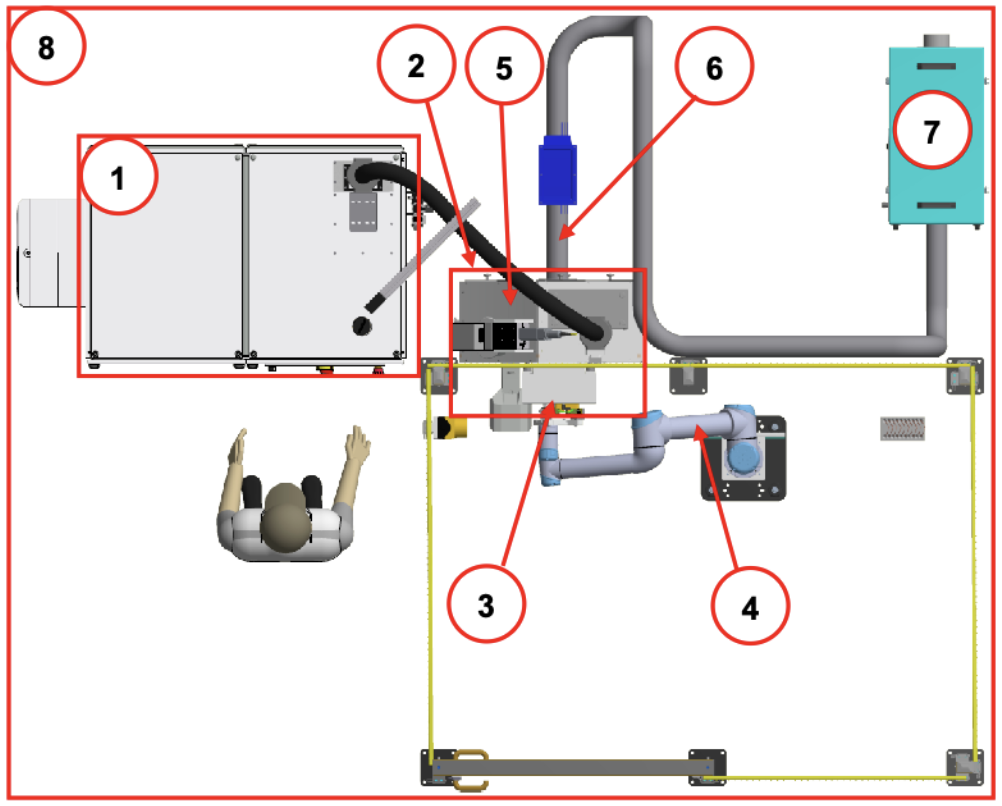
\includegraphics[width=0.8\textwidth]{figs/AbsiolierZelle.png}
  \caption{Gesamtansicht des Laserbearbeitungssystems, \cite[Abb.~2.1, S.~19]{CleanLaser2022}}
  \label{fig:laser_system_aufbau}
\end{figure}
%
Der markierte Punkt 1 ist der Serverschrank, in dem viele Teile der Laseranlage verbaut sind. Die 2.
zeigt die Schutzeinhausung des Lasers, die Nummer 5 ist die optische 2D-Laseroptik. All diese Subsysteme
werden im Folgenden genauer beschrieben.
Der Roboterarm (4) führt die Hairpins in den individuellen Schutzdeckel (3). Für einen sicheren Betrieb
ist zudem eine Absaugung (7) über Schläuche an die Schutzeinhausung angebracht (6). Diese sorgt für eine
Absaugung der entstandenen Partikel beim Abisolieren.
Weiter ist in der \cref{fig:laser_system_aufbau} der Arbeitsbereich des Roboterarmes durch einen Zaun begrenzt.
Diese Zelle sorgt für eine sichere Benutzung der Anlage. Die Maße dieser Zelle sind mit \todo{Maße der Zelle!}
fest vorgegeben. In \cref{fig:AufbauAbisolierZelle} ist zudem eine Aluminium-Extrusions-Struktur, bei der
es möglich ist Subsysteme zu montieren, die für den Roboterarm zu erreichen sind. Der Aufbau befindet sich in der
gegenüberliegenden Ecke zum Laser, also in der \cref{fig:laser_system_aufbau} unten rechts. Hier werden
bereits die unten beschriebenen Trays, usw. montiert.

\begin{figure}[htbp]
	\centering
	    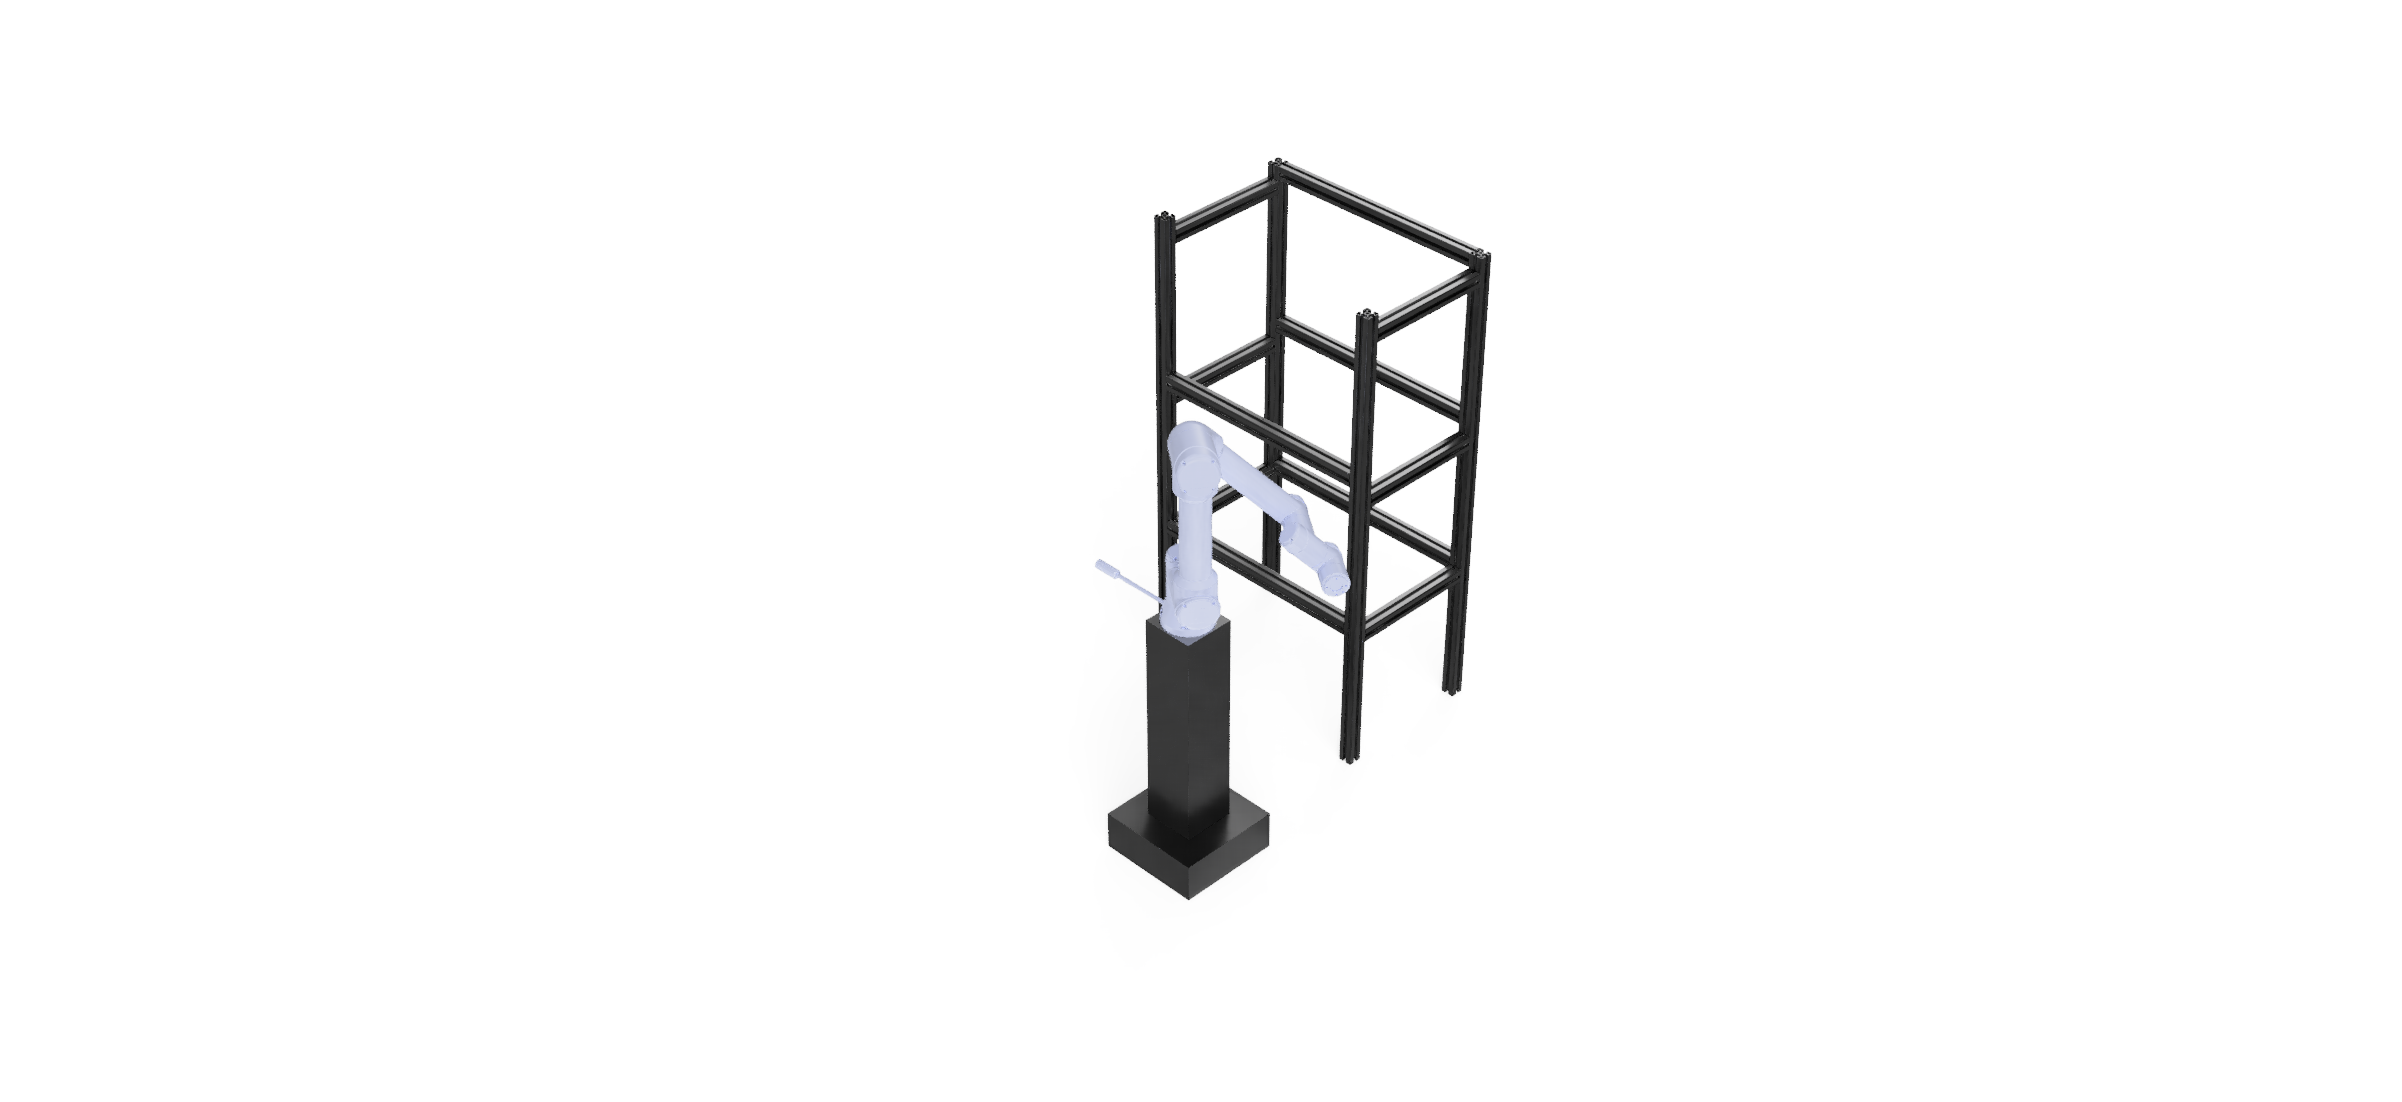
\includegraphics[width=1\linewidth]{figs/AufbauAbisolierZelle.png}
	\caption{Aufbau der Abisolierzelle mit Roboterarm und Laser}
	\label{fig:AufbauAbisolierZelle} 
\end{figure}
%
%
\subsubsection{Clean-Laser-Anlage}\label{sec:CleanLaser}
Die Clean-Laser-Anlage ist für den eigentlichen Schritt der Abisolierung der Hairpins verantwortlich.
Dafür wird ein Laserstrahl verwendet, der die Enden der Hairpins so bearbeitet, dass die Abisolierung
abgetragen wird.

Das Laserbearbeitungssystem ist eine Sonderanfertigung des Herstellers, welches einen CL 300GR Laser
mit Optik Stamp 14 und einem Prozessmodul. Dieses Gesamtsystem wird wireLine MIRROR static genannt,
da der Laserstrahl so aufgeteilt werden muss, dass alle vier Seiten des Hairpins bearbeitet werden können.\\

Die Laseremitierung ist bei diesem System in einem externen gekühlten Serverschrank, in dem auch
weitere Versorgungseinheiten, wie der Industrie PC zur Steuerung, eine pneumatische Regelungsanlage und
Siemens ET200SP Signalklemmen als Kommunikationsschnittstellen, verbaut sind. Der Laser ist
als diodengepumpter Festkörperlaser ausgelegt, der mit 300W besonders beschädigungsarm metallische
Bauteile bearbeiten kann. Die optische Strahlungsleistung ist so hoch, dass die Isolierung wie PEEK, PI und PAI\todo{Abkürzungsverzeichnis}
optimal entfernt werden können. Weiter ist zu beachten, dass dieses System der Laserklasse 4 angehört und
mit dem 1064nm Infrarotlaserstrahl für Menschen unsichtbar ist. Dies birgt Sicherheitsrisiken, die aber durch
passende Schutzeinrichtungen und einer dementsprechenden Steuerung minimiert werden können.\\

Nach dem Bereitstellen des Laserstrahls, wird dieser durch einen optischen Leiter in die Schutzeinhausung
der eigentlichen Abisoliereinrichtung geführt. Hier wird der Laserstrahl durch Spiegel so abgelenkt, dass
alle vier Kanten des zu bearbeitenden Hairpins erreicht werden können.
Dazu gibt es zu den festverbauten Spiegeln in der Schutzeinhausung in der Laseroptik an sich (Stamp 14)
die Möglichkeit den Laserstrahl in 2D, also X- und Y-Richtung, zu bewegen. In \cref{fig:laser_MIRROR_system} sieht man,
dass diese Strahlenablenkung genutzt wird, um mit einem einmaligen Ausrichten der Spiegel, jeden Punkt am Hairpin zu erreichen.
Der Vorteil dabei ist, dass keine vier Laser für jede Kante benötigt werden.
Außerdem wird mit dem benötigten Gehäuse dieses System nun als Produkt der Laserklasse 1 klassifiziert.

Das Sicherheitssystem besteht aus vielen Sensoren, die einen sicheren Betrieb gewähren. So gibt es
Notschalter, einen Türsensor und Metalldetektoren, die den Verschluss aller Serviceklappen und Ausgänge bestätigen.
Eine Vielzahl an weiteren Kontrollmechanismen geben dem Bedienelement und schlussendlich der Steuereinheit
Rückschluss auf den Status des Systems. Die Bedienung, erfolgt dabei durch die Erstellung eines eigenen Programmes
und der Aktivierung dessen durch einen Fußknopf. Weiter ist es möglich den Befehl des Abisolierens durch einen
externen Eingang, wie den Roboterarm, durchzuführen.
\begin{figure}[htbp]
  \centering
  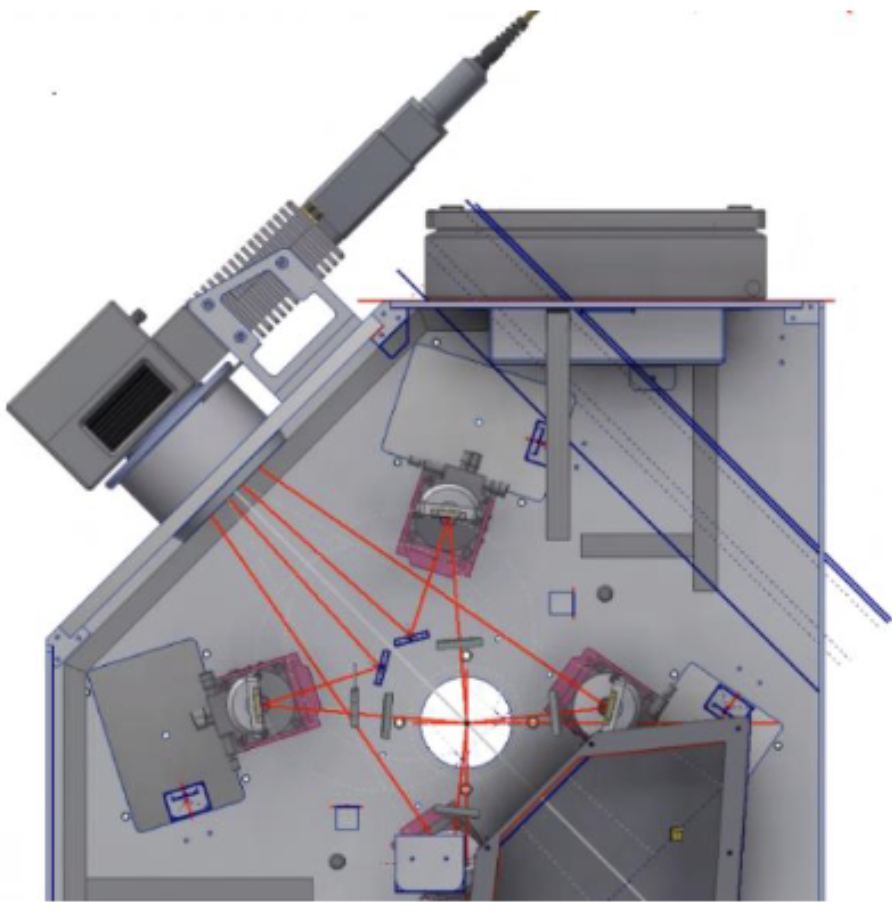
\includegraphics[width=0.4\textwidth]{figs/wireLine MIRROR.png}
  \caption{wireLINE MIRROR System - Laserstrahlführung, \cite[Abb. Bearbeitungsoptik, S.~42]{CleanLaser2022}}
  \label{fig:laser_MIRROR_system}
\end{figure}

\todo{- Wie lange braucht ein Durchlauf?}
%
%
\subsubsection{Universal Robots Roboterarm}\label{sec:UniversalRobot}
Der vorhandene Roboterarm ist ein 6-Drehgelenkarm von Universal Robots. Der UR5e hat eine maximale Nutzlast
von 5\,kg. Als Endeffektor steht ein Greifersystem mit zwei pneumatisch betriebenen Linearaktuatoren zur Verfügung. Diese sind
wiederum, je nach Hairpin-Form, so positioniert, dass mit einem Plastikaufsatz der Kupferdraht richtig gegriffen wird.\\
Die Steuerung und Programmierung erfolgt durch einen externen Touchscreen, auf dem mittels einer GUI passende
Blöcke aufeinander geschoben werden oder einfach Einstellungen betätigt werden. Die pneumatische Steuerung des Endeffektors
erfolgt durch die Verbindung einer Festo-Valve und den programmierbaren digitalen Ausgängen des Roboterarms.
Die Wiederholgenauigkeit liegt bei ungefähr $\pm 0{,}03$\,mm und die Gelenke können sich maximal um 360° drehen.
\PEMfootcite{ur5e_handbuch_2025}\\

%
\subsubsection{Gesamtverfahren}\label{sec:GesamtVerfahrenAktuell}
Der bisherige Arbeitsablauf bestand bei diesem System daraus, dass Hairpins vorbereitet wurden, diese dann in
der Zelle platziert wurden, der Roboterarm kalibriert und aktiviert wurde. Der letzte Schritt bestand dann
nach dem Abisolieren im Laser die Hairpins in eine Ablage zu geben.

Dieses System basiert auf manuellen Eingriffen in wichtigen Schritten des Prozessflusses. So müssen für
jede Hairpin-Art eigene Trays montiert werden, in denen die Hairpins gehalten werden können. Aktuell sind
diese einfache Aluminiumextrusionen mit montierten Füßen, die vorher im 3D-Drucker erstellt wurden. Der Bedienende
muss nun nach einem Durchlauf von circa 10 Hairpins den Roboterarm deaktivieren und in der Zelle neue Hairpins
platzieren. Erst danach kann der Roboterarm wieder aktiviert werden und ein weiterer Durchlauf der Abisolierung
starten. Dies bringt zwei große Probleme mit sich:\\
1. kein kontinuierlicher Prozessfluss,\\
2. Rekalibrierung der Position der Hairpins,\\
3. Anpassung der Trays an jede Hairpin-Art.\\

Der erste Punkt ist direkt ersichtlich und folgt durch die Pause, die entsteht, wenn der Bedienende die Zelle
betreten muss. Der zweite Punkt, muss nach jeder Inbetriebnahme geschehen, da sich die Trays verschieben können
oder sich die Längen der Hairpins verändern. Außerdem müssen die Trays jedes Mal für den Hairpin passend vorhanden
sein. Ist dies nicht der Fall muss eine neue Version erstellt und gedruckt werden. Dies bedeutet einen 
weiteren Schritt im Prozess, der für das Umbauen benötigt wird.

Die weiteren Schritte, wie die Bewegungen des Roboterarmes und die Abisolierung, erfolgen voll automatisch
durch ein vorher definiertes Programm. Dieses ist einfach anpassbar und arbeitet über feste Taktzeiten.
Die Ablage der Hairpins erfolgt durch ein einfaches Übergeben des Roboterarmes auf eine Führung für Hairpins.
Besondere Hairpin-Arten, wie die I-Pins unterliegen ähnlichen Arbeitsschritten, wobei die Trays und die Ablage
anders aufgebaut sind. 
%
%
\subsection{Existierende Produktionen}\label{sec:RealeProduktionen}
- Wie sehen aktuelle Serienproduktionen aus? Was ist der Unterschied zu Prototypenproduktion?\\
- Welche Technologien werden eingesetzt?\\
- Welche Taktzeiten werden erreicht? Welche Kosten entstehen? An einem Beispiel zeigen\\
%
%
\subsection{Subsystem-Betrachtung}\label{sec:SubSystem}
Die oben beschriebenen Anlagen lassen sich jeweils in mehrere Subsysteme unterteilen. Zur Analyse
der verschiedenen Auslegungsmöglichkeiten wird die VDI 2860\PEMfootcite{VDI2860.1990} - Handhabungsfunktion benutzt. Diese
Richtlinie wurde 2018 wegen einer teilweise veralteten Betrachtung zurückgezogen, ist aber für diesen
Abschnitt dennoch relevant mit zu betrachten.

In der Handhabungstechnik wird nämlich in die Teilfunktionen Speichern, Mengen verändern, Bewegen, Sichern
und Kontrollieren unterschieden. Genau diese Themen werden im Folgenden detailliert betrachtet und analysiert.
%
\subsubsection{Lagerung}\label{sec:LagerungsSystem}
Es gibt drei unterschiedliche Lagerarten:\PEMfootcite{MontageIndustriellenProduktion.2012}\\
1. Ungeordnete Speicherung - Bunkern,\\
2. Teilgeordnete Speicherung,\\
3. Geordnete Speicherung - Magazinieren.\\
Das erste System wird in den meisten Fällen für Kleingut, welches schon in einem unsortierten Zustand 
angeliefert wird, verwendet. Die Teile liegen also einfach als Schüttgut vor. Wichtig ist hier zu beachten,
dass diese zwar ungeordnet sein dürfen aber nicht mit anderem Kleingut durchmischt werden. Vorteile eines
solchen Systems sind die kostengünstige Befüllung sowie eine hohe Speicherdichte und damit die große Puffermenge
an Teilen. Auf der anderen Seite muss das Schüttgut meistens für den weiteren Produktionsprozess sauber
geordnet werden. Hier entstehen typische Probleme wie das Verhaken der Teile untereinander oder ein möglicher
Abrieb.

Die teilgeordnete Speicherung ist ein Kompromiss aus beiden Welten. Hier sind die Teile in einer Dimension
angeordnet. Sie sind also z. B. liegend auf einer Ebene orientiert und können so einfacher entnommen werden.
Dies wird sehr häufig in Kombination mit der flexiblen Entnahme durch einen bildverarbeitungsgestützten Roboterarm
mit passendem Greifer genutzt. Vorteile sind dabei die Vielfältigkeit der Teile, die mit dem passenden Greifer verwendet
werden können. Als Nachteil ist wiederum, das ständige gezielte Nachfüllen von Teilen und einer im Vergleich zu
anderen Systemen langsamen Taktzeit. Die größte Störgröße der letzten beiden Systeme ist jedoch die sogenannte Brückenbildung,
die eine Behinderung für die weitere Produktion darstellt. 

Die \cref{fig:zufuehrprinzipien} zeigt den groben Aufbau der
drei typischsten Ausführungen der beiden ersten Systeme auf. Für die Lagerung mittels Bunker, sind diese Systeme meist 
mit einer direkten Einheit zum Ordnen der Teile ausgeführt. Der Vibrationsförderer (a) benutzt dabei Vibrationen,
um das Kleingut auf einer kontrollierten Bahn zu bewegen. Diese Bahn kann aufgrund ihrer Größe und Beschaffenheit nur maximal ein Teil tragen.
So werden die Teile als geordnete Reihe aus dem System gegeben. Ähnlich funktioniert der Stufenförderer (b), wo 
die Teile einzeln Stück für Stück angehoben werden. Dabei haben die einzelnen Treppen ebenfalls die passende Größe,
sodass auch hier die Teile geordnet ausgegeben werden. Es muss aber nochmal gesagt sein, dass zumeist ein weiteres System
zur richtigen Orientierung der Teile benötigt wird. Das modernste und technisch komplexeste System, ist die
flexible Zuführung (c), die durch Kameraalgorithmen und einer präzisen Steuerung eines Greifers eine geordnete Entnahme ermöglicht. 
Häufig muss die Lagefläche mit einem Backlight und einer Vibrationsmöglichkeit ausgelegt
werden, damit die Erkennung und Bereitstellung von freiliegenden Teilen gewährleistet werden kann.

\begin{figure}[htbp]
\centering
\begin{tikzpicture}[
  font=\scriptsize,
  part/.style={draw, fill=black!15, minimum width=2.6mm, minimum height=1.3mm,
               inner sep=0pt, outer sep=0pt},
  fl/.style={-{Stealth[length=1.8mm]}, thick},
  thin fl/.style={-{Stealth[length=1.4mm]}},
  lbl/.style={align=center, font=\scriptsize}
]

%% ---------------- (a) Vibrationswendelförderer ----------------
\begin{scope}[shift={(0,0)}]
  \draw[thick] (0.35,0) -- (0.05,2.0);
  \draw[thick] (2.15,0) -- (2.45,2.0);
  \draw[thick] (0.35,0) -- (2.15,0);
  \draw[gray] (0.30,0.35) -- (2.20,0.55);
  \draw[gray] (0.24,0.85) -- (2.26,1.05);
  \draw[gray] (0.18,1.35) -- (2.32,1.55);
  \node[part] at (0.75,0.44) {};  \node[part] at (1.55,0.52) {};
  \node[part] at (0.95,0.96) {};  \node[part] at (1.80,1.06) {};
  \node[part] at (1.30,1.48) {};
  \node[part, rotate=25] at (0.85,0.14) {};
  \node[part, rotate=-40] at (1.35,0.16) {};
  \node[part, rotate=70] at (1.75,0.13) {};
  \draw[fl] (1.15,1.72) -- (2.05,1.80);
  \draw[thick] (2.45,1.90) -- (3.05,1.70);
  \draw[thick] (2.38,1.62) -- (2.95,1.44);
  \node[part] at (2.72,1.68) {};
  \draw[thin fl] (3.05,1.60) -- (3.35,1.48);
  \foreach \x in {0.55,1.25,1.95}{
    \draw[gray] (\x,0) -- ++(0.18,-0.30) -- ++(-0.18,-0.20) -- ++(0.18,-0.25);
  }
  \draw[thick, fill=black!8] (0.30,-0.95) rectangle (2.20,-0.75);
  \draw[{Stealth[length=1.3mm]}-{Stealth[length=1.3mm]}, gray]
        (2.55,-0.55) arc (-20:20:1.1);
  \node[gray, right=0.5mm] at (2.75,-0.20) {Schwingung};
\end{scope}

%% ---------------- (b) Stufenförderer ----------------
\begin{scope}[shift={(5.15,0)}]
  \draw[thick] (0.0,2.0) -- (0.45,0.15) -- (1.05,0.15);
  \node[part, rotate=15] at (0.45,0.30) {};
  \node[part, rotate=-35] at (0.72,0.32) {};
  \node[part, rotate=55] at (0.58,0.55) {};
  \node[part, rotate=-10] at (0.80,0.62) {};
  \draw[thick] (1.05,0.15) -- (1.05,0.55) -- (1.50,0.55);
  \draw[thick] (1.50,0.55) -- (1.50,0.95) -- (1.95,0.95);
  \draw[thick] (1.95,0.95) -- (1.95,1.35) -- (2.40,1.35);
  \draw[thick] (2.40,1.35) -- (2.40,1.75) -- (2.85,1.75);
  \node[part] at (1.27,0.62) {};  \node[part] at (1.72,1.02) {};
  \node[part] at (2.17,1.42) {};  \node[part] at (2.62,1.82) {};
  \foreach \x in {1.30,1.75,2.20}{
    \draw[{Stealth[length=1.3mm]}-{Stealth[length=1.3mm]}, gray] (\x,0.20) -- (\x,0.42);
  }
  \node[gray, align=center] at (1.75,-0.02) {Hubbewegung};
  \draw[thick] (2.85,1.75) -- (3.35,1.58);
  \draw[thin fl] (3.20,1.48) -- (3.50,1.36);
\end{scope}

%% ---------------- (c) Flexible Zuführung ----------------
\begin{scope}[shift={(10.30,0)}]
  \draw[thick] (0.0,1.95) -- (0.30,1.30) -- (0.72,1.30);
  \node[part, rotate=30] at (0.28,1.48) {};
  \node[part, rotate=-20] at (0.48,1.44) {};
  \draw[thin fl] (0.52,1.22) -- (0.62,0.85);
  \draw[thick, fill=black!5] (0.15,0.45) rectangle (3.05,0.62);
  \node[gray, below=0.5mm] at (1.60,0.45) {Backlight-Fläche};
  \node[part, rotate=20] at (0.60,0.72) {};
  \node[part, rotate=-55] at (1.05,0.70) {};
  \node[part, rotate=80] at (1.45,0.73) {};
  \node[part, rotate=-15] at (1.95,0.70) {};
  \node[part, rotate=45] at (2.45,0.72) {};
  \draw[thick, fill=black!10] (1.35,2.05) rectangle (1.95,2.35);
  \draw[thick] (1.55,2.05) -- (1.55,1.92) -- (1.75,1.92) -- (1.75,2.05);
  \node[above=0.3mm] at (1.65,2.35) {Kamera};
  \draw[gray, dashed] (1.55,1.90) -- (0.70,0.78);
  \draw[gray, dashed] (1.75,1.90) -- (2.55,0.78);
  \draw[thick] (2.60,1.85) -- (2.60,1.45);
  \draw[thick] (2.42,1.45) -- (2.78,1.45);
  \draw[thick] (2.42,1.45) -- (2.42,1.15);
  \draw[thick] (2.78,1.45) -- (2.78,1.15);
  \draw[thin fl] (2.60,1.98) -- (2.60,2.30);
  \node[above=0.3mm] at (2.60,2.30) {Roboter};
  \draw[{Stealth[length=1.3mm]}-{Stealth[length=1.3mm]}, gray] (0.75,0.28) -- (1.35,0.28);
\end{scope}

\node[lbl] at (1.65,-1.55) {(a) Vibrationswendelförderer};
\node[lbl] at (6.90,-1.55) {(b) Stufenförderer};
\node[lbl] at (12.05,-1.55) {(c) Flexible Zuführung};

\end{tikzpicture}
\caption[Prinzipskizzen ausgewählter Zuführprinzipien]{Prinzipskizzen ausgewählter
Zuführprinzipien: (a) ungeordnete Bevorratung mit mechanischer Ordnung durch
Schikanen, (b) schonende, stufenweise Förderung aus dem Bunker, (c) teilgeordnete
Bereitstellung mit kamerabasierter Lageerkennung und Direktgriff. Eigene
Darstellung in Anlehnung an \cite{GrundlagenHandhabungstechnik.2020}.}
\label{fig:zufuehrprinzipien}
\end{figure}
%
Im Gegensatz zu den eben beschriebenen Systemen zur Lagerung von unsortierten Teilen, geht es im Folgenden um die Lagerung und Bereitstellung
von Teilen die in einem bereits geordneten Zustand vorliegen. Die sogenannte Magazinierung bedarf einer genauen Anpassung
an die jeweiligen Teile\PEMfootcite{Werkstueckmagazin.2008}. In \cref{fig:magazinbauformen} sind sechs der gängigsten
Magazinsysteme für sperrige Teile, wie Hairpins, dargestellt. In der ersten Skizze (a) ist ein Schachtmagazin dargestellt, 
bei dem die Teile in einem senkrechten Schacht gelagert werden. Mit einem Schieber lässt sich definiert ein Teil entnehmen.
Die Schwerkraft sorgt für ein Nachrücken der Teile. Als Vorteil hierbei ist die Möglichkeit der Speicherung
einer großen Menge an Teilen und die einfache Entnahme zu nennen. Da Brückenbildungen oder Verhaken der Teile ein häufiges
Problem darstellt, ist meist ein externer Rüttelmechanismus oder Spannfeder notwendig.

Das Reihen- oder Hängemagazin (b) profitiert bei passenden Teilen von einem sehr einfachen Aufbau. Dabei stehen oder hängen
die Teile in einer Schiene. Ein Nachführen erfolgt entweder durch das Anschrägen der Schiene und somit das Nutzen der Schwerkraft.
Eine andere Möglichkeit wäre ebenfalls ein Vibrationsmechanismus, der die Teile in eine definierte Richtung bewegt.
Vorteil bei diesem System ist geringe Verhakungs- und Beschädigungsgefahr. Im Gegensatz steht dazu die im Vergleich geringe
Speicherkapazität an Teilen, da die Länge des Magazins schnell ansteigt.

Das Trommelmagazin (c) wird meist als Schnittstelle zwischen zwei Subsystemen genutzt. Die Teile werden auf der einen Seite 
auf die Fläche abgelegt und diese dann in jedem Taktschritt in eine Richtung weiterbewegt. Dies funktioniert in einer sehr
kompakten und prozesssicheren Bauart. Es wird aber ein externer Antrieb vorausgesetzt und die Taktung muss mit den
anliegenden Systemen übereinstimmen. Außerdem ist wegen der kompakten Bauform und dem Umfang der Trommel die Kapazität
begrenzt.

Das Kettenmagazin (d) basiert auf einem ähnlichen Prinzip zum Reihen- oder Hängemagazin, nur dass hier statt die Teile
dicht aneinandergereiht zu speichern, jedes Teil eine eigene Halterung bekommt. Diese Werkstückträger sind auf einer
umlaufenden Kette montiert. Ähnlich wie beim Trommelmagazin bewegen sich die Träger je Taktschritt in eine definierte Richtung,
mit dem Vorteil die Abstände und Menge der Träger frei zu skalieren. Auch ist es bei einer entsprechenden Überwachung
unterschiedliche Bauarten der Teile aufzunehmen. Die Herausforderungen sind dabei aber ein hoher mechanischer Aufwand und
der dementsprechende erhöhte Verschleiß der einzelnen Komponenten.

Das in (e) skizzierte Palettenmagazin oder auch Traysystem gibt es in sehr unterschiedlichen Ausführungen. So können
die Teile liegend in einzelnen Nestern oder auch stehend in einer Reihe gespeichert werden. Dabei ist aber bei jeglicher
Bauform wichtig, dass jedes Teil an einer bekannten Position in einer vordefinierten Lage abgelegt wird. Hierbei sticht besonders
die teilschonende und fest definierte Lageposition heraus. Auf der anderen Seite müssen diese Trays vorbereitet und bestückt
werden.

Das letzte System, der Werkstückgurt (f), wird häufig in der Magazinierung von elektrischen Komponenten verwendet. Dieser
Ansatz wird zwar meistens für kleinere Bauteile verwendet, ist aber in einem modifizierten Aufbau, in dem nicht das gesamte
Bauteil, sondern nur ein kleiner Teil, vom Gurt eingeschlossen wird auch in Betracht zu ziehen. Normalerweise sind die
Komponenten jeweils in einem verschlossenen Container verstaut, der für eine hohe Prozesssicherheit und Teilschonung sorgt.
Auch hier muss eine solche Rolle vorbereitet oder von extern bezogen werden. Dies lohnt sich erst ab hohen Stückzahlen.

\begin{figure}[htbp]
\centering
\begin{tikzpicture}[
  font=\scriptsize,
  wp/.style={draw, fill=black!15, minimum width=3.2mm, minimum height=1.4mm,
             inner sep=0pt, outer sep=0pt},
  fl/.style={-{Stealth[length=1.7mm]}, thick},
  tf/.style={-{Stealth[length=1.4mm]}, gray},
  lbl/.style={align=center, font=\scriptsize}
]

%% ---- (a) Schachtmagazin ----
\begin{scope}[shift={(0,0)}]
  \draw[thick] (0.55,0.30) -- (0.55,2.60);
  \draw[thick] (2.05,0.30) -- (2.05,2.60);
  \foreach \y in {0.55,0.85,1.15,1.45,1.75,2.05,2.35}{
    \draw[fill=black!15] (0.62,\y) rectangle (1.98,\y+0.17);
  }
  \draw[tf] (2.45,2.35) -- (2.45,1.05);
  \node[gray, rotate=90, anchor=south] at (2.62,1.30) {Schwerkraft};
  \draw[thick, fill=black!8] (0.30,0.05) rectangle (1.20,0.25);
  \draw[fl] (1.30,0.15) -- (2.20,0.15);
\end{scope}

%% ---- (b) Reihen-/Hängemagazin ----
\begin{scope}[shift={(5.20,0)}]
  \draw[thick] (0.20,2.30) -- (3.05,2.30);
  \foreach \x in {0.55,1.05,1.55,2.05,2.55}{
    \draw[thick] (\x-0.14,2.28) -- (\x-0.14,1.72)
      arc (180:360:0.14) -- (\x+0.14,2.28);
  }
  \draw[fl] (0.70,2.62) -- (2.40,2.62);
  \node[gray] at (1.55,1.25) {geordnet, lagedefiniert};
  \draw[tf] (2.70,2.05) -- (3.10,2.05);
\end{scope}

%% ---- (c) Trommelmagazin ----
\begin{scope}[shift={(10.40,0)}]
  \begin{scope}[shift={(1.55,1.55)}]
    \draw[thick] (0,0) circle (0.92);
    \draw[thick] (0,0) circle (0.30);
    \foreach \a in {0,45,...,315}{ \draw[gray] (\a:0.30) -- (\a:0.92); }
    \foreach \a in {22,67,112,157,202,247,292}{
      \node[wp, rotate=\a] at (\a:0.62) {};
    }
    \draw[{Stealth[length=1.5mm]}-, thick] (1.10,0.35) arc (30:-30:1.25);
  \end{scope}
  \node[gray] at (2.95,0.95) {Takt};
  \draw[tf] (1.55,0.50) -- (1.55,0.12);
\end{scope}

%% ---- (d) Kettenmagazin ----
\begin{scope}[shift={(0,-3.75)}]
  \draw[thick, rounded corners=0.55cm] (0.45,0.65) rectangle (2.75,2.35);
  \foreach \x in {0.95,1.60,2.25}{
    \node[wp] at (\x,2.35) {};
    \node[wp] at (\x,0.65) {};
  }
  \node[wp, rotate=90] at (0.45,1.50) {};
  \node[wp, rotate=90] at (2.75,1.50) {};
  \draw[fl] (1.20,2.62) -- (2.05,2.62);
  \draw[tf] (3.05,1.50) -- (3.45,1.50);
\end{scope}

%% ---- (e) Palettenmagazin / Tray ----
\begin{scope}[shift={(5.20,-3.75)}]
  \draw[thick] (0.30,0.65) rectangle (3.00,2.35);
  \foreach \x in {0.975,1.65,2.325}{ \draw[gray] (\x,0.65) -- (\x,2.35); }
  \foreach \y in {1.2166,1.7833}{ \draw[gray] (0.30,\y) -- (3.00,\y); }
  \foreach \x in {0.6375,1.3125,1.9875,2.6625}{
    \foreach \y in {0.94,1.50,2.07}{ \node[wp] at (\x,\y) {}; }
  }
  \node[gray] at (1.65,0.30) {ortsfeste Nester};
\end{scope}

%% ---- (f) Werkstückgurt ----
\begin{scope}[shift={(10.40,-3.75)}]
  \draw[thick] (0.85,1.50) circle (0.62);
  \draw[thick] (0.85,1.50) circle (0.16);
  \draw[thick] (0.85,2.12) -- (3.10,2.12);
  \draw[thick] (0.85,1.82) -- (3.10,1.82);
  \foreach \x in {1.35,1.85,2.35,2.85}{ \node[wp] at (\x,1.97) {}; }
  \draw[fl] (1.60,2.45) -- (2.60,2.45);
  \node[gray] at (1.85,1.20) {Rolle};
  \draw[tf] (3.20,1.97) -- (3.55,1.97);
\end{scope}

\node[lbl] at (1.30,-0.55) {(a) Schachtmagazin};
\node[lbl] at (6.75,-0.55) {(b) Reihen-/Hängemagazin};
\node[lbl] at (11.95,-0.55) {(c) Trommelmagazin};
\node[lbl] at (1.60,-4.30) {(d) Kettenmagazin};
\node[lbl] at (6.85,-4.30) {(e) Palettenmagazin (Tray)};
\node[lbl] at (12.00,-4.30) {(f) Werkstückgurt};

\end{tikzpicture}
\caption[Bauformen geordneter Magazine]{Bauformen geordneter Magazine zur
lagedefinierten Bevorratung von Werkstücken. Eigene Darstellung in Anlehnung
an \cite{GrundlagenHandhabungstechnik.2020}.}
\label{fig:magazinbauformen}
\end{figure}

Diese Magazinsysteme haben jeweils unterschiedliche Anforderungen an Vorbereitung und Nachbearbeitung. Ziel ist jedoch
jedes Mal, dass die Bauteile in einer geordneten Lage zwischengespeichert werden können. Je nach Anwendung und System
kommen die Magazine entweder schon vorbestückt durch den Produzenten oder müssen erst durch ein weiteres System befüllt
werden. Neben der manuellen Bestückung kann dies beispielsweise durch erweiterte Systeme wie die in \cref{sec:LagerungsSystem}
beschriebenen passieren. Bei jedem dieser Systeme muss jedoch betrachtet werden, wie die Bauteile in ein weiteres Subsystem übergeben
werden. Häufig muss das Bauteil als vereinzeltes Stück übergeben werden, was bei den Magazinen außer dem Reihen- und Hängemagazin
der Fall ist. Auch die Lagerungssysteme müssen zur weiteren Verwendung vereinzelt werden. Die Betrachtung solcher Systeme folgt
in \cref{sec:VereinzelungSystem}.
%
%
\todo{Hairpin spezifischer???}
\todo{- Welche Positionen müssen die Hairpins haben?
- Wie können die Hairpins "gespeichert" werden?
- Wie wird dafür gesorgt, dass nichts verhakt?}
%
\subsubsection{Vereinzelung}\label{sec:VereinzelungSystem}
Nach der VDI 2860 braucht es für viele Prozesse eine Abtrennung von Werkstücken aus einem geordneten Strom. Genau für diesen
Zweck gibt es unterschiedliche mechanische Ansätze\PEMfootcite{RNAAutomation.o.J.}. Ein häufig verwendeter Mechanismus ist dabei
die Vereinzelung mittels Schieber. Ähnlich wie bei dem in \cref{sec:LagerungsSystem} beschriebenen Schachtmagazin, wird das Bauteil
so aus dem System geschoben, dass immer nur ein Bauteil zur Zeit dieses verlässt. 

Eine andere Möglichkeit ist es das Bauteil in eine Vorrichtung zu befördern, in der nur exakt ein Bauteil reinpasst. Diese
Vorrichtung mit einem Bauteil kann dann so verschoben werden, dass dieses nun vereinzelte Bauteil freigegeben wird. Wird dieser
Prozess in einer bestimmten Taktzeit wiederholt, lässt sich eine robuste und einfache Vereinzelung ermöglichen.

An das eben beschriebene System orientiert sich auch das Zellenrad. Auch hier gibt es passende Auskerbungen, sodass nur ein einzelnes
Bauteil Platz findet. Der Vorteil hierbei, ist dass es möglich ist auch aus einem unsortierten Lager Bauteile zu nehmen. Da die Formen
auf dem Rad jeweils nur einen Platz haben, lässt sich auch so eine Vereinzelung ermöglichen.

Die variableste Art der Vereinzelung beschreibt aber die Vereinzelung durch Sperrklinken. Bei dieser Methode wird auf zwei gegeneinander
arbeitende Sperrfinger gesetzt, die sequenziell versetzt arbeiten. Im ersten Moment sperrt der vordere Arm und Bauteile
bewegen sich so weit vor, bis diese auf den versperrten Weg treffen. Nun kann je nach Anforderung der zweite Arm zwischen zwei
Bauteile ausfahren und so eine vorher eingestellte Anzahl an Bauteilen isolieren. Fährt nun der vordere Arm ein, kann das isolierte
Bauteil im nächsten System verwendet werden. Dieses Prinzip bietet die Möglichkeit flexibel die Anzahl der zu vereinzelnden
Bauteile durch den Abstand der beiden Arme einzustellen.

\todo{Was sind Vor- und Nachteile?}
%
\subsubsection{Transport}\label{sec:TransportSystem}
Damit Bauteile von einem Subsystem in ein Anderes gelangen, bedarf es der Wahl eines passenden Transportsystems. Es muss auf
Taktrate, Fehlerquote und Ausfallsicherheit geachtet werden. Für die Untersuchung der folgenden Ausführungen
wurde zwischen aktiven und passiven Transportsystemen unterschieden.

Als Voraussetzung für ein passives Transportsystem gilt, dass dieses System ohne Zufuhr von externer Steuerung und Energie
funktioniert. Die Schwerkraft spielt in diesem Zusammenhang eine wichtige Rolle, da diese durch eine vorliegende Höhendifferenz
Bauteile bewegen kann. Die häufigsten Ausführungen dieses Systems sind Rutschen oder Fallschächte, über die die Bauteile geführt
über eine Ebene gleiten. Ein solcher Aufbau muss individuell an das Bauteil angepasst sein, wobei aber immer eine Höhendifferenz
zwischen den Schnitt- und Übergabepunkten vorhanden sein muss. Außerdem muss für eine Bewegung physikalisch der passende Grenzwinkel
zum Überwinden der Haftreibung\PEMfootcite{Reibung.2001} eingestellt sein:
\begin{equation}
  \tan(\alpha) = my_(H)
\end{equation}
Da im Normalfall die Gleitreibung kleiner als die Haftreibung ist, wird mit dieser Formel also der Winkel zwischen dem vertikalen 
Boden und der schiefen Ebene beschrieben. Die Konstante muss individuell zwischen der Werkstoffpaarung, also zwischen Außenschicht des
Bauteils und Beschaffenheit der schiefen Ebene. Der steilste Winkel beschreibt die Aufstellung im rechten Winkel mit einem Winkel von 90°.
Hierbei ist aber zu beachten, dass dieser theoretische Wert in der Praxis selten verwendet wird, weil besonders bei kleineren Bauteilen
die Gefahr besteht, dass sich diese überschlagen und in einer unerwünschten Lage ankommen. Weiter ist mit diesem System eine
Geschwindigkeitskontrolle schwer möglich. Denn es muss verhindert werden, dass sich Bauteile verharken oder die Haftreibung nicht überwinden können.
Dafür bedarf es einer gewissen Geschwindigkeit, die für die Minderung solcher Probleme tendenziell höher gewählt wird. Dies wiederum kann
zu Beschädigungen, wie Verformungen oder Abrieb, führen. Auf der anderen Seite ist ein solches System einfach im mechanischen Aufbau,
kostengünstig und eine wartungsarme Methode die Schnittstellen der einzelnen Subsysteme zu verbinden.

Die folgenden Transportsysteme setzen auf einen externen Antrieb, zählen also zu den aktiven Systemen. Der Vibrationslinear-
und Bandförderer kommen aber trotzdem ohne eine elektronische Regelung aus. Es kann ausschließlich zwischen den zwei Zuständen
AN und AUS entschieden werden. Der Vibrationslinearförderer benutzt Vibrationen bei einer festen Frequenz, die die Bauteile in
Mikroschritten vorbewegen. Physikalisch werden die Teile bei jeder Amplitude eine minimale Strecke weiter geworfen. Passiert dies
mit der zum Bauteil passenden Frequenz und Amplitude, stellt sich eine kontinuierliche gerade Bewegung ein. Dieses System ist sehr
robust und in der Industrie viel vertreten, da die Bewegung in einer moderaten konstanten Geschwindigkeit passiert. Auch lassen sich
mit einer dedizierten Steuerung weitere Parameter in einem gewissen Rahmen anpassen. Neben der einfachen Funktionsweise stellt aber
besonders die Lautstärke des Systems und ein recht komplexer Aufbau mit vielen Komponenten Probleme dar.
Die wohl bekannteste und gängigste Art der Transportsysteme sind die Förderbänder. Diese gibt es in einer großen Variation bezüglich
Bauteilart, Größe und Geschwindigkeit. Grundsätzlich werden die zu befördernden Teile aber liegend auf einem Band abgelegt.
Dabei gibt es einen Punkt bei dem Teile dazu gegeben werden und einen Endpunkt an dem diese wieder abgegeben werden. Das Band besteht
meistens aus einem runden kontinuierlichen Kunststoffband, welches über zwei Umlenkrollen rotiert. Die Oberseite wird so zu einer
linear bewegten Ebene, die durch Spannung der Rollen oder weitere Führungsräder eben gehalten wird. Diese bewährte Lösung bietet
neben ihrer Variantenvielfalt auch die Möglichkeit einer weiteren Regelung, um ebenfalls Parameter wie Geschwindigkeit und Taktzeit
dem benötigten Prozess anzupassen. Nachteil ist die Wartbarkeit, da in diesem System viele unterschiedliche bewegbare Komponenten
verbaut werden.

Die in \cref{fig:wirkkette-antrieb} dargestellten Linearachsen sind eine weitere Möglichkeit Bauteile zu bewegen. Der Zahnriemen-Ansatz
ist dabei verwandt zu den gerade beschriebenen Förderbändern. Der Spindel- und Zahnstangenansatz soll hierfür noch einmal genauer
betrachtet werden, denn diese bieten den Vorteil extrem präzise Positionen anzufahren. Laut Altintas werden besonders die Kugelgewindegetriebe
verwendet \PEMfootcite{Altintas.2011}. Diese ist eine kleine mechanische Änderung gegenüber der Spindel, bei der statt einer Mutter
eine lange Reihe an Kugeln um das Gewinde der Welle geführt wird. So wird die Rotation der Spindel in eine abnutzungsarme und energieeffiziente
Vor- und Rückbewegung des Läufers umgewandelt. Trotz der höheren Komplexität des mechanischen Aufbaus sind die Vorteile bei einer
dauerhaften Nutzung relevant. Außerdem nur für diese Antriebe nicht nur die externe Energiequelle in Form eines Motors zu berücksichtigen,
sondern auch eine vorhandene aktive Regelung. Da diese Antriebe durch zwei Endpunkte begrenzt sind, muss die Regelung dafür sorgen,
dass der Schlitten innerhalb dieses Bereiches bleibt. Dieses System kann weiter auch für eine genaue Positionierung genutzt werden,
welches individuelle Anfahrten für den Schlitten ermöglicht.

Alle diese beschriebenen Systeme müssen für den jeweiligen Einsatz stark angepasst werden. Es gibt noch einige weitere Transportsysteme,
die auf anderen Antrieben, wie elektromagnetische Linearantriebe oder selbstfahrbare Wägen für Industriehallen. Diese wurden aber
hier nicht weiter betrachtet, da diese nur unwahrscheinlich für den Hairpintransport und diese Arbeit in Betracht gezogen werden können.
\todo{Definition Transportsystem? Schnittstellenübergabe...}
%
\subsubsection{Fixierung}\label{sec:FixierungSystem}
Für die Bearbeitung oder Übergabe an neuen Subsystemen, bedarf es einer passenden Fixierung von Bauteilen. Es lässt sich grob in Kraftschluss-
und Formschluss-Fixierungssysteme unterscheiden. Für die sehr schonende Art der Formschlussfixierung kommen an das Bauteil angepasste
Konturen und Halter zum Einsatz. Diese sind so konstruiert, dass die Bauteile ohne eine externe Halterung in ihrer Position bleiben. Da
nur Auflagekräfte wirken, ist eine mechanische Beeinflussung des Bauteils sehr unwahrscheinlich. Das Dimensionieren und Designen
eines solchen Systems bedarf jedoch einer intensiven Prüf- und Konstruktionsphase. Es muss für jedes Bauteil eine teiletypgebundene
Version erstellt werden, welches eine Variation von Bauteilen entgegenspricht.

Die andere Möglichkeit ist der Kraftschluss, bei dem ein externer Fixiermechanismus zum Einsatz kommt. Das Bauteil wird so an definierten
Stellen eingespannt und gehalten. Für den genauen Aufbau eines solchen Mechanismus gibt es eine Vielzahl unterschiedlicher Ansätze, \todo{Das als Quelle?: https://www.mechstream.com/clamping-mechanism-motion-animations/}
wobei meistens Backen an das Bauteil unter Druck angesetzt werden. Da eine genaue Betrachtung der unterschiedlichen Aufbauten, den
Rahmen sprengen würde, wird später in der Realisierung die konkrete Umsetzung beschrieben. Problem dieses Systems ist aber, dass
eine Krafteinwirkung auf das Bauteil zu Beschädigungen und Verformungen führen kann. Wird dies im Konstruktionsprozess nicht mit
beachtet, sind die Vorteile wie die Möglichkeit verschiedene Bauteile aufzunehmen nicht mehr relevant.

Eine gesonderte Art der Kraftschlussmechanismen sind Greifersysteme, die hier noch einmal gesondert aufgeführt werden, da das bereits
in \cref{sec:AktuellesSystem} dargestellte System ein solches beinhaltet. Auch hier gibt es eine große Variation von mechanischen Aufbauten,
wobei hier meist linear bewegbare Backen verwendet werden. Für die Fixierung und Bewegung werden elektromechanische oder pneumatische
Antriebe verwendet. Ein solches Gesamtsystem besteht dabei aber wieder aus mehreren Subsystemen\PEMfootcite[Abbildung 9]{Strasser.2011}. 
Es wird unterschieden in den Greifer, also dem Wirk-/Haltesystem ansich, dem Antriebssystem für die Bewegung der Fixierung, einem Tragsystem
an dem die einzelnen Greifer montiert sind, ein Steuerungssystem mit Sensorfeedback und ein Schutz- und Sicherheitssystem für die Anlage
selber und das Bedienpersonal.

Weiter gibt es noch Vakuumgreifer oder magnetische Halterungen, die aber wegen ihrer sehr individuellen Anwendung in dieser Arbeit
nicht detaillierter betrachtet werden müssen.
%
%
\subsubsection{Positionierung}\label{sec:PositionierungsSystem}
In diesem Abschnitt sollen Systeme analysiert werden, die die Positionierung von Hairpin und dessen Halterung kontrollieren. Dazu kann
zwischen kontinuierlichen Wegsensoren und inkrementellen Sensoren mit Referenzpunkten unterschieden werden. Die in \cref{sec:Sensorik}
beschriebenen Sensoren dienen hauptsächlich zur Überprüfung, ob ein Hairpin an einer bestimmten Position vorbeigekommen ist. Diese Sensortypen
werden im späteren Verlauf dieser Arbeit eingesetzt und verglichen.

Eine kontinuierliche Sensoreinheit zeichnet sich dadurch aus, dass diese zu jeder Zeit einen absoluten Wert ausgibt, der die Position
widerspiegelt. Auch nach einem vorherigen Ausschalten ist dieses System in der Lage, die Position direkt als kontinuierlichen Wert
auszugeben. In der Industrie werden hierfür zumeist Potentiometer verwendet, die bei einem Verschieben eine veränderte kontinuierliche
Spannung ausgeben. Dies folgt dem einfachen Spannungsteiler-Prinzip: Über die gesamte Sensorlänge mit fest definiertem Widerstand wird eine
Versorgungsspannung angelegt. Auf diesem Bereich wird nun ein Abnehmer platziert, der mit der zu bestimmenden Position des Schlittens
verbunden ist. Ändert sich nun die Position des Abnehmers, verändert sich auch das Widerstandsverhältnis und damit die Spannung am Abnehmer.
\begin{equation}
  U_(Abnehmer) = U_(Versorgung) * R_(GND/Abnehmer) / (R_Gesamt)
\end{equation}
Die Endpunkte bilden einmal die niedrigste Spannung am Ground mit 0V und die höchste Spannung am Ende des Widerstandes mit der Versorgungsspannung.
Für eine lineare Bewegung wird meist ein länglicher Widerstand verwendet. Es gibt aber auch Potentiometer in Rundausführung, die
aber dem gleichen elektrischen Prinzip entsprechen. Der Vorteil dieses Prinzips, ist die einfache Kopplung an eine elektrische Regelung,
da wie bereits erwähnt nur eine einfache analoge Spannung mit Umrechnung als Positionssignal gilt. Dieses schnelle und direkte Signal
ist mit dem einfachen Aufbau kaum anders zu realisieren. Bei einem dauerhaften Betrieb stellen sich jedoch Probleme beim Verschleiß
heraus, da der Abnehmer durch den ständigen mechanischen Druck und das Bewegen den Kontakt immer weiter abnutzt.

Bei den inkrementellen Sensoren unterscheidet man in open-loop und closed-loop. Diese unterscheiden sich im Feedback an die Regelung.
Grundsätzlich wird hierbei mit End- oder Referenzpunkten gearbeitet. Zur Initialisierung des Systems müssen dafür bestimmte Sensoren,
meist Endschalter, angefahren werden, damit einmalig eine feste Position vorgegeben wird. Hier gibt es eine weitere Trennung für die
Steuerung an sich: Für open-loop Systeme reicht die Anfangsposition und die vorgegebenen Bewegungen werden intern verrechnet. Bei
einem Antrieb mit Schrittmotor z. B. werden nur die einzelnen Schritte vorgegeben. Die Gefahr hierbei ist, dass wegen Überlast einzelne
Schritte ohne registriert zu werden übersprungen werden. Dies wiederum führt dazu, dass die Steuerung nach diesem Schritt eine
zur Realität abweichenden Position annimmt. Wird dieses System jedoch in seinen Arbeitsbereichen betrieben, treten solche Ungenauigkeiten
selten auf und das System ist mechanisch und elektrisch einfach aufzubauen.
Dem Gegenüber steht das closed-loop System, bei dem die Steuerung auf einen weiteren Kontrollmechanismus zurückgreifen kann. Dieser
gibt durch elektrische Zähler, meist in Form von Hall-Sonden, die die Magnetfeldänderung durch die Rotation in Motoren zählen können
die genaue Schrittanzahl wieder. So können Fehler zurückgerechnet werden und die berechnete Position der Steuerung stimmt immer mit
der realen Position überein. Als Nachteil ist hier klar der zusätzliche Aufwand durch weitere Komponenten und Schnittstellen zu nennen.
%
%
\subsection{Forschungslücke}\label{ResearchGap}
Nach Vorstellung dieser ganzen Systeme, stellt sich heraus, dass es eine Vielzahl an Möglichkeiten gibt den mechanischen und elektrischen
Aufbau dieser Arbeit zu gestalten. In der Produktion ist eben dies die Herausforderung, eine passende Anlage für einen genauen Verwendungszweck
zu entwickeln. Besonders die Prototypenproduktion mit Anforderungen, wie das Verarbeiten verschiedener Hairpin-Geometrien, stellt
eine so hohe Individualisierung heraus, dass eine solche Anlage nicht frei auf dem Markt erhältlich ist. Eben aus diesem Grund muss
geprüft werden, ob der Bau einer solchen Anlage überhaupt möglich ist und im Dauerbetrieb Vorteile mit sich bringt.
\todo{Besseren Titel verwenden?}

\newpage
\section{Lösungsansatz}\label{sec:loesungsansatz}
Dieser Abschnitt beschreibt einen der größeren Teile der Arbeit. Hier soll detailliert gezeigt werden, wie das System
zur automatischen Abisolierung in der Prototypenproduktion aussehen soll und welche Entscheidungen auf diesem Weg
getroffen wurden.\\
Dafür sollten noch einmal grob die Anforderungen und Bedingungen dargelegt werden:\\
Das System, das entwickelt werden soll, muss in der Lage sein, aus einer hängenden Reihe von Hairpins einzelne dieser
an den Roboter zu übergeben. Dabei dürfen die Hairpins nicht beschädigt werden und die Übergabe an den Roboterarm
muss mit einer festen Taktzeit und einer hohen Wiederholgenauigkeit geschehen.\\
Zunächst musste sich ein grober Aufbau einer solchen Anlage angesehen werden. Dafür wurden zwei primäre zu erledigende
Arbeitsschritte festgelegt:\\
1. Die Vereinzelung der Hairpins,\\
2. Die Auslieferung und Übergabe eines einzelnen Hairpins an den Roboterarm.\\
Der genaue Aufbau dieser Subsysteme wird im späteren Teil dieses Abschnittes weiter erläutert. Zunächst muss man sich
einen Überblick über die technischen Möglichkeiten verschaffen. Es wird in drei grobe Kategorien unterteilt:\\
- die mechanischen Bauteile \\
- die elektronischen Komponenten \\
- die Programmierung/der Code \\


Es gibt drei Themenbereiche der Anlage:
1. Die Vereinzelung der Hairpins,
2. Die Auslieferung des Hairpins zum Roboter,
3. Das Greifen und Abisolieren des Hairpins mittels Roboterarm, wobei diese Aufgabe nicht Teil dieser Arbeit ist.

\subsection{Mechanische Bauteile}\label{sec:Mechanik}
In diesem Teil werden mechanische Bauteile, die für ein solches System benötigt werden, untersucht. Relevant
sind dabei besonders die Punkte wie Einsetzbarkeit, Langlebigkeit und Praktikabilität.
%
\subsubsection{Aktuatorik}\label{Aktuatorik}

%
\subparagraph{Pneumatik}
%
\subparagraph{Elektronische Aktuatorik}
-Servomotor
-Spindel
-Belt driven
-Roboterarm?
%
%
\subsubsection{Material}\label{sec:MaterialAuswahl}
PLA
%
\subsubsection{Aluminiumprofile}\label{sec:AluProfil}
%
%
\subsection{Elektronische Komponenten}\label{sec:ElektronischeKomponenten}
%
\subsubsection{Spannungsversorgung}\label{sec:SpannungsVersorgung}
%
\subsubsection{Microcontroller}\label{sec:Microcontroller}
%
\subsubsection{Sensorik}\label{sec:Sensorik}
%
\subsubsection{Motoren}\label{sec:Motoren}
%


\subsection{CodeStruktur}\label{sec:CodeStruktur}
Welche Code-Strukturen gibt es für Ausfallsicherheit etc.? Welche Code-Struktur wird verwendet? Welche Vorteile und Nachteile hat diese Code-Struktur?

\subsubsection{Aktuelle Systeme aus der Produktion}\label{sec:Codesystems}
Welche Normen und Arten für solche Systeme gibt es?

\subsubsection{Code-Struktur der Anlage}\label{sec:CodeStrukturAnlage}
Diagramm für Signalfluss, Fallbacks, Sicherheit


\subsection{Vereinzelung}\label{sec:Vereinzelung}
Das Subsystem der Vereinzelung muss die Hairpins mit einer hohen Taktzeit
und Zuverlässigkeit vereinzeln. Dabei muss aus einem Bündel von Hairpins ein
einzelner Hairpin ausgegeben werden.
%
\subsection{Auslieferung}\label{sec:Auslieferung}
Das Subsystem der Auslieferung muss die Hairpins mit einer hohen Taktzeit
und Zuverlässigkeit ausliefern.
\newpage
\section{Realisierung}\label{sec:Realisierung}
Wie wurde die Anlage aufgebaut?
%
%
\subsection{Verwendete Tools}\label{sec:VerwendeteTools}
- Kurze Vorstellung ALLER verwendetn Tools:\\
Fusion360, GitHub, BambuLab, KI für Codeentwicklung
%
\subsection{Hardware}\label{sec:Hardware}
- Wie wurde das System physisch aufgebaut?\\
%
\subsection{Software}\label{sec:Software}
- Wie wurde das System vom Code her aufgebaut?\\
%
\subsection{Herausforderungen \& Probleme}\label{sec:ChallengesProbleme}
- Was waren die größten Herausforderungen?\\
- Welche Probleme gab es?\\
%
\newpage
\section{Validierung und Tests}\label{sec:ValidierungTests}
%
%
\subsection{Verifikation der Subsysteme}\label{sec:VerifikationSubsysteme}
\todo{Allgemeiner Testaufbau}
%
\subsubsection{Vibrationseinheit}
\todo{Messaufbau, Egrebnisse}
%
\subsubsection{Sperrklinken}
\todo{Messaufbau, Egrebnisse}
%
\subsubsection{Transportsystem}
\todo{Messaufbau, Egrebnisse}
%
\subsubsection{Fixierungssytem}
\todo{Messaufbau, Egrebnisse}
%
%
\subsection{Systemtest im Gesamtablauf}\label{sec:Systemtest}
%
\subsubsection{Versuchsaufbau und Durchführung}\label{sec:Versuchsaufbau}
- Wie werden die Tests gemacht?\\
- Worauf muss geachtet werden?\\
- Welche Testreihen werden gemacht?\\
%
\subsubsection{Versuchsreihe Taktzeit}\label{sec:VR_Taktzeit}
- Tabelle, etc. für Versuchsreihe nach Prüfung der Taktzeit\\
%
\subsubsection{Versuchsreihe Wiederholgenauigkeit}\label{sec:VR_Wiederholgenauigkeit}
- Tabelle, etc. für Versuchsreihe nach Prüfung der Wiederholgenauigkeit\\
%
\subsubsection{Versuchsreihe Dauerlauf}\label{sec:VR_Durchsatz}
- Tabelle, etc. für Versuchsreihe nach Optimierung/Änderung des Durchsatzes von verarbeiteten Hairpins\\
%
\subsubsection{Versuchsreihe Beschädigung}\label{sec:VR_Beschädigung}
- Tabelle, etc. für Versuchsreihe nach Prüfung der Beschädigung/Veränderung der Hairpins\\
%
%
\subsection{Fehlerbetrachtung}\label{sec:Fehlerbetrachtung}
- Einschätzung der eintretenden Fehler!\\
%
%
\subsection{Bewertung gegen Anforderungsliste}\label{sec:Testbewertung}
- Vergleich gegen Anforderung\\
\todo{Vergleich gegen vorherigen Prozess!}


%\subsection{Ausfall-Betrachtung}\label{sec:Ausfall}
%- Was passiert, wenn ein Subsystem, Spannungsversorgung versagt?\\
%- FMEA Betrachtung!\\
%- Sicherheitsregeln für Produktionsanlagen?\\


\newpage
\section{Optimierungen & Fazit}\label{sec:Fazit}
Hier steht die Zusammenfassung und der Ausblick.
At vero eos et accusam et justo duo dolores et ea rebum.

\subsection*{Optimierungen}\label{sub:Optimierungen}
Lorem ipsum dolor sit amet, consetetur sadipscing elitr, sed diam nonumy eirmod tempor invidunt ut labore et dolore magna aliquyam erat, sed diam voluptua. At vero eos et accusam et justo duo dolores et ea rebum. Stet clita kasd gubergren, no sea takimata sanctus est Lorem ipsum dolor sit amet. Lorem ipsum dolor sit amet, consetetur sadipscing elitr, sed diam nonumy eirmod tempor invidunt ut labore et dolore magna aliquyam erat, sed diam voluptua. At vero eos et accusam et justo duo dolores et ea rebum. Stet clita kasd gubergren, no sea takimata sanctus est Lorem ipsum dolor sit amet.

\subsection*{Fazit}\label{sub:Fazit}
Lorem ipsum dolor sit amet, consetetur sadipscing elitr, sed diam nonumy eirmod tempor invidunt ut labore et dolore magna aliquyam erat, sed diam voluptua. At vero eos et accusam et justo duo dolores et ea rebum. Stet clita kasd gubergren, no sea takimata sanctus est Lorem ipsum dolor sit amet. Lorem ipsum dolor sit amet, consetetur sadipscing elitr, sed diam nonumy eirmod tempor invidunt ut labore et dolore magna aliquyam erat, sed diam voluptua. At vero eos et accusam et justo duo dolores et ea rebum. Stet clita kasd gubergren, no sea takimata sanctus est Lorem ipsum dolor sit amet.
\newpage

%TODO: Bestimmte Editoren, wie TeXstudio highlighten TODO-Kommentare was während der Erstellung eines Dokuments sehr nützlich sein kann.


\appendix
%% Römische Numerierung
% Mit diesem Befehlssatz kann die Nummerierung des Anhangs auf Röhmische Zahlen umgestellt werden. Empfohen wird dies nicht, weil z. B. "VIII" deutlich mehr platz einnimt, als "C" und damit die Einrückung im Inhaltsverzeichnis sehr groß werden muss.
%Setz die Kapitelzahl auf 5 (Inhaltsverzeichnis ist I, Formelzeichen II usw.
% Achtung: Der Zähler begind bei 0. D.h. Inhaltsverzeichnis = I entspricht Zähler = 0)
%\renewcommand{\theHsection}{\thesection}
%\sectionnumbering{Roman} 



\begingroup
\raggedright
\sloppy
\printbibliography
\endgroup

\newpage

%Anhang
\section{Anhang}
\begin{figure}[htbp]
	\centering
	    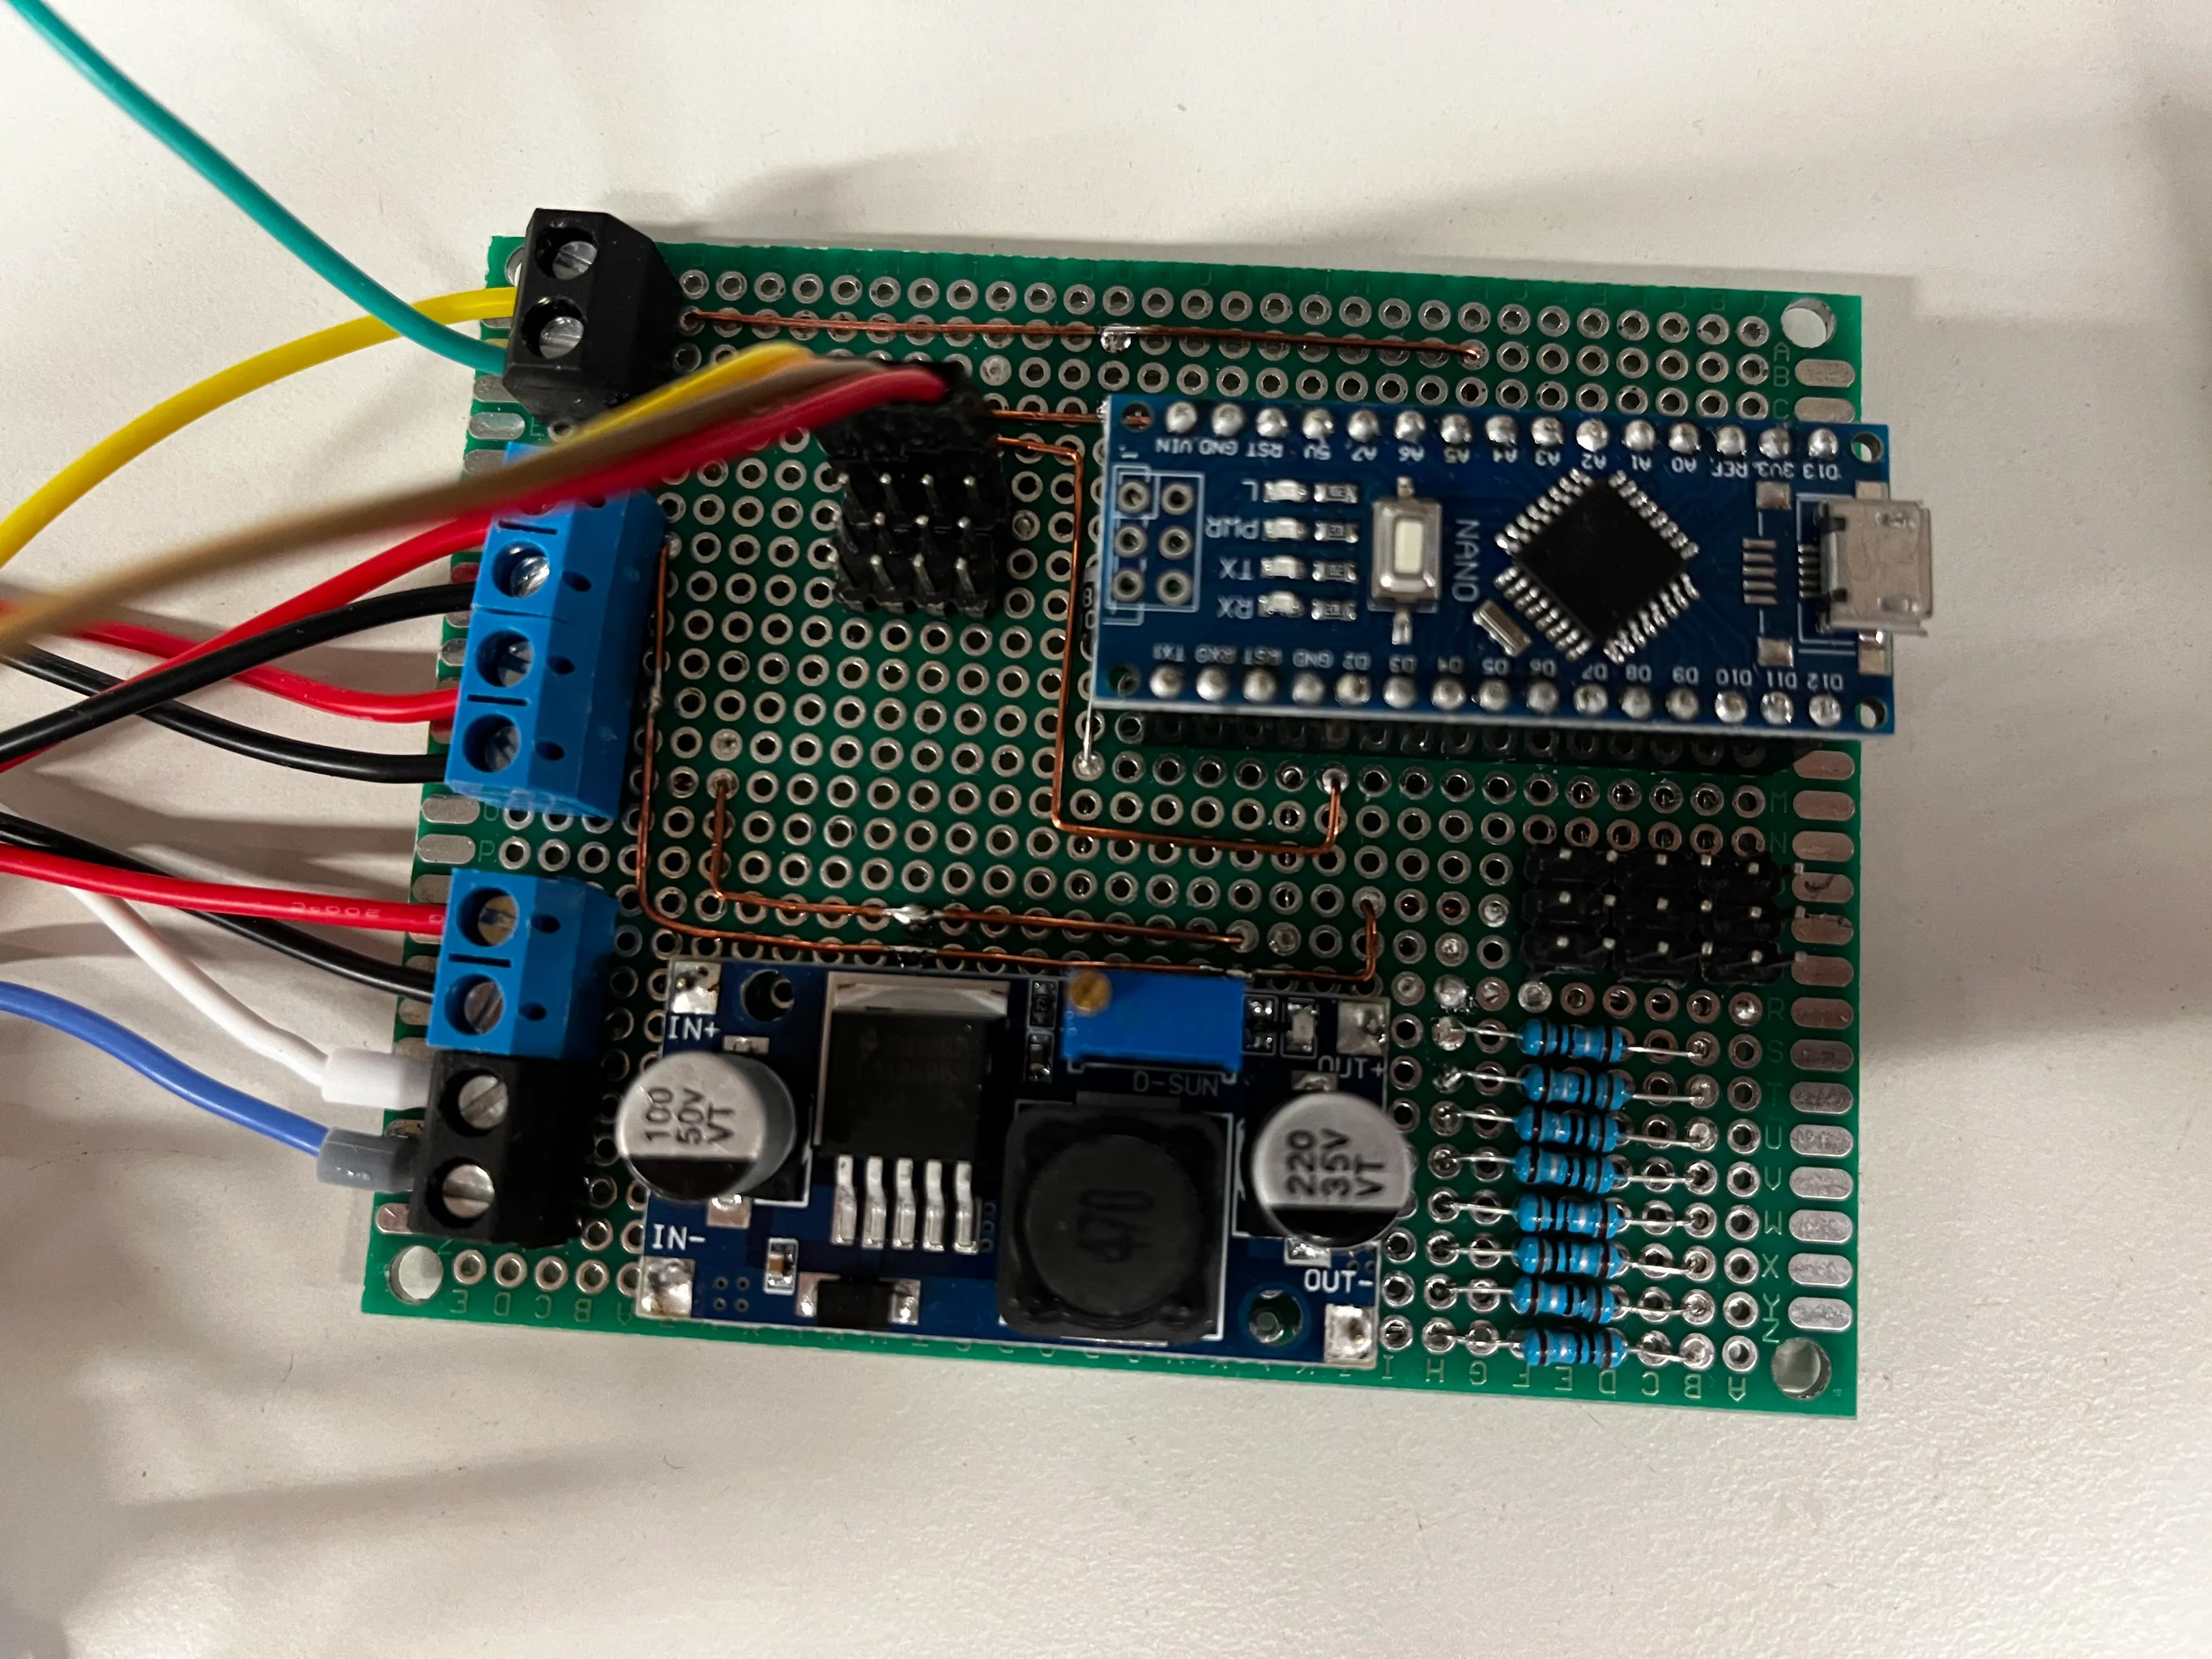
\includegraphics[width=0.8\linewidth]{figs/Lochraster_Nano.png}
	\caption{Aufbau der Lochrasterplatine mit dem Arduino Nano}
	\label{fig:Lochraster_Nano}
\end{figure}

\newpage

%Erklärung
\sffamily
	\section{Eidesstattliche Versicherung}
Hinweise zur Eidesstattlichen Versicherung sind hier zu finden:
\url{http://www.rwth-aachen.de/cms/root/Studium/Im-Studium/Pruefungen-Abschlussarbeiten/~hjxv/Hinweise-zu-schriftlichen-Arbeiten/}

Sollte eine in \LaTeX{} gesetzte Version benötigt werden, kann ggf. die nachfolgend auskommentierte Version als Basis genutzt werden.

%\large
%
%\vspace{1cm}
%\textbf{Mustermann, Maximilian} \hfill \textbf{Matrikelnummer: 000000}
%\vspace{1cm}
%
%\noindent
%Ich versichere hiermit an Eides Statt, dass ich die vorliegende Bachelorarbeit mit dem Titel "`\colorbox{red}{Hier Titel der Arbeit einfügen}"' selbstständig und ohne unzulässige fremde Hilfe erbracht habe. Ich habe keine anderen als die angegebenen Quellen und Hilfsmittel benutzt. Für den Fall, dass die Arbeit zusätzlich auf einem Datenträger eingereicht wird, erkläre ich, dass die schriftliche und die elektronische Form vollständig übereinstimmen. Die Arbeit hat in gleicher oder ähnlicher Form noch keiner Prüfungsbehörde vorgelegen.
%
%\vspace{1.75cm}
%
%\noindent
%\begin{tabularx}{\linewidth}{lXl}
%	\makebox[5cm]{\hrulefill} & \hfill & \makebox[5cm]{\hrulefill} \\
%	Ort, Datum                &        & Unterschrift
%\end{tabularx}
%\vfill
%\small
%\raggedright
%\textbf{Belehrung:}\\
%\textbf{\S 156 StGB: Falsche Versicherung an Eides Statt}\\
%Wer vor einer zur Abnahme einer Versicherung an Eides Statt zuständgien Behörde eine solche Versicherung falsch abgibt oder unter Berufung auf eine solche Versicherung falsch aussagt, wird mit Freiheitsstrafe bis zu drei Jahren oder mit Geldstrafe bestraft.\\
%\vspace{0.5cm}
%\textbf{\S 161 StGB: Fahrlässiger Falscheid; fahrlässige falsche Versicherung an Eides Statt}\\
%(1) Wenn eine der in den \S\S 154 bis 156 bezeichneten Handlungen aus Fahrlässigkeit begangen worden ist, so tritt Freiheitsstrafe bis zu einem Jahr oder Geldstrafe ein.\\
%(2) Staflosigkeit tritt ein, wenn der Täter die falsche Angabe rechtzeitig berichtigt. Die Vorschriften des \S 158 Abs. 2 und 3 gelten entsprechend.\\
%\large
%\vspace{0.2cm}
%Die vorstehende Belehrung habe ich zur Kenntnis genommen:\\
%\vspace{1.75cm}
%\begin{tabularx}{\linewidth}{lXl}
%	\makebox[5cm]{\hrulefill} & \hfill & \makebox[5cm]{\hrulefill} \\
%	Ort, Datum                &        & Unterschrift
%\end{tabularx}
%

\normalfont

\end{document}

